%
%
%   NISHIMURA
%
%

% 11/14 14:22 nakayama が編集しました。
% 11/16 0:30 edited by nishimura
% 11/16 6:00 edited by nakayama
% 11/24 11:00 edited by nishimura


\documentclass[11pt,b5paper,papersize,dvipdfmx]{jsbook}
% \documentclass[11pt,b5paper,papersize,dvipdfmx,draft]{jsbook}

\usepackage{vuccaken}
\usepackage{vuccaken2018}
\usepackage{11nsmr}

\begin{document}

% - - - - - - - - - - - - - - - - - - - - - - - - - - -
\kaishititle{音とサインとそれからイヤホン♪}{物理科学科3回生}{西村宗悟}
% - - - - - - - - - - - - - - - - - - - - - - - - - - -

%
\section{はじめに}
今回の私の会誌のテーマは音です。音が伝わることは身近な物理現象でありながら音の研究をする人が少なく、たくさんの人に音響工学の面白さを伝えたいと思い会誌のテーマを音しました。なるべく物理学初学者の方にもわかりやすいように書いたので、気軽に読んでいただけると思います。\par
音の簡単な分析に挑戦してみることを目標にして、まずは音とは何かを説明しました。その後、音の解析に関連する事柄を中心に話をしつつ、実際に周期的な音である矩形波を周期的な関数に見立てて、数学的な手法のフーリエ級数展開を用いて解析しました。次に実際にフリーソフトの「WaveGene」を用いて矩形波を作り、それをフリーソフトの「WaveSpectra」で周波数解析して、周期的な関数のフーリエ変換と比較しました。
最後にフリーソフトの「Audacity」を用いて、人間の言語の音の解析を行いました。\par
おまけとして、イヤホンの種類などについて書いたので興味がある方は読んでください。(イヤホンの話と今回のテーマである音の話は関係ありません(笑))

%%
\section{音って何ですか?}
%
\subsection{音の基礎}
私たちはたくさんの音に囲まれて生活をしています。
外を歩けば風の音や車の走る音が聞こえますし、室内でも冷暖房設備の稼働音や換気扇の回る音などが
常に聞こえてきますよね。
では、音とはいったい何なのでしょうか?\par
音とは何かを一言で言うと、気体・液体・固体を媒質として伝わる振動のことです。
日常生活で使われる音という単語は人間の聴覚で知覚できる振動のことを指しますが、厳密に言えば媒質を振動が伝わるもの全てを音と言うので、人間の聴覚が知覚できない媒質の振動でもその振動を音といいます。具体的には周波数$20\sim20000\tani{Hz}$の波が人間の聴覚が知覚できる音です。\par
音が伝わるというのはどういう現象なのでしょうか? 
音が伝わるのは媒質を構成する分子の振動がある粒子からある粒子に伝わる現象です。
また、媒質が振動するというのは圧力が変動することと置き換えることができるので、
音は圧力変動が伝わる現象とも考えられます。
%
\subsection{音の大きさって何?}
音は媒質の振動であり、その振動によって空気の圧力が変動します。その圧力の変動の大きさを音圧といいます。音圧は大気圧と同じく空気の圧力なので、音圧の単位は$\tani*{Pa}$ (パスカル)を用います。
\begin{itembox}[l]{圧力}
  圧力とは単位面積当たりに加わる力の大きさのことです。$1\tani{Pa}$は以下のように定義されます。
  \begin{align}
    1\tani{Pa}=\frac{1\tani{N}}{1\tani{m^2}}
  \end{align}
  ここで$1\tani{N}$は$1\tani{kg}$の物体に$1\tani{m/s^2}$の加速度を生じさせるための力の大きさです。
\end{itembox}\par
人によっても異なりますが、人間が音を感じる最小の音圧は$20\tani{\mu Pa}$、
最大の音圧(音よりも痛みの方が強くなる音圧)は$20\tani{Pa}$程度です。
大気圧は約$1013\tani{hPa} \,(\approx 10^5\tani{Pa})$であるので、人間の耳が感じる音圧の大きさはとても小さいです。\par
ここまで、音圧$\tani*{Pa}$のお話をしてきましたが、我々が普段テレビなどで耳にする音の大きさは$\tani*{dB}$ (デシベル)を単位にしていますよね? 実は、音の大きさとして用いているのは音圧レベルというものです。まずは音圧レベルの定義を求めることを目標に話を進めていきます。\par
最初に音の強さを定義します。音の強さは単位面積を1秒間で通過する音のエネルギーであり、以下のように定義されます。
\begin{itembox}[l]{音の強さ}
  その点における音の強さを$I$、音圧を$p$とします。
  \begin{align}
    I=\frac{p^2}{\rho c} \tani*{W/m^2}\label{fig:ototuyosa}
  \end{align}
  ここで$\rho$は空気の密度$\sim 1.2\tani{kg/m^3}$、$c$は音速$\sim 340\tani{m/s}$です。
\end{itembox}

{\noindent\bf 式(\ref{fig:ototuyosa})の証明(次元解析)}\par
上式の関係において、もちろん右辺と左辺の次元は一致しないといけません。ここからは左辺の単位と右辺の単位が等しくなるかどうかを確かめます。
方針としては、左辺は単位面積を1秒間で通過する音のエネルギーを音の強さと定義したので、右辺が果たして
音のエネルギーの単位と一致するかを確かめます。\par
$\tani*{W}$は仕事率の単位です。仕事率とは単位時間あたりにどれだけの仕事をするかを表すものです。
仕事の単位はエネルギーの単位と同じく$\tani*{J}$であり、仕事は加わっている力$\tani*{N}$と
その力をかけ続けている間に移動した距離$\tani*{m}$の積で書けます。
\begin{align}
  \mathrm{J} = \mathrm{N} \cdot \mathrm{m}
\end{align}
また、力$\tani*{N}$はニュートンの運動方程式より(力を加える物体の質量)$\tani*{kg}$と
(動いているときの加速度)$\tani*{m/s^2}$の積で書けるので、
\begin{align}
  \mathrm{N} = \mathrm{kg} \cdot (\mathrm{m/s^2})
\end{align}
以上の関係を用いて$\mathrm{W}$を$\mathrm{m}$,\,$\mathrm{kg}$,\,$\mathrm{s}$の単位で表すと、
\begin{align}
  \mathrm{M}&= \frac{\mathrm{J}}{\mathrm{s}}
  = \frac{ \mathrm{N} \cdot \mathrm{m} }{ \mathrm{s} }\nonumber\\
  &= \frac{( \mathrm{kg}\cdot \mathrm{m/s^2} ) \cdot \mathrm{m}}{\mathrm{s}}\nonumber\\
  &= \frac{\mathrm{kg}\cdot \mathrm{m^2}}{\mathrm{s^3}}
\end{align}
式(\ref{fig:ototuyosa})の右辺の単位を次元解析すると
\begin{align}
  \text{(式(\ref{fig:ototuyosa})の右辺の単位)}
  &= \frac{\mathrm{Pa}^2}{ (\mathrm{kg/m^3})(\mathrm{m/s}) }\nonumber\\
  &= \frac{ (\mathrm{N/m^{2}})^2 }{ (\mathrm{kg/m^3})(\mathrm{m/s}) }\nonumber\\
  &= \frac{ \mathrm{N^2}\cdot \mathrm{s} }{ (\mathrm{m}^2\cdot \mathrm{kg}) }\nonumber\\
  &= \frac{
        ( \mathrm{kg} \cdot (\mathrm{m/s^2}) )^2 \cdot \mathrm{s}
      }{
        ( \mathrm{m^2} \cdot \mathrm{kg} )
      } \nonumber\\
  &= \qty( \mathrm{kg} \frac{\mathrm{m^2}}{\mathrm{s^3}} )\frac{1}{ \mathrm{m^2} }\nonumber\\
  &= \frac{ \mathrm{W} }{ \mathrm{m^2} }
\end{align}
以上より、式(\ref{fig:ototuyosa})の右辺と左辺の次元が一致することを示せました。\par

次に音の強さのレベル表示をします。
人間が音を感じる場合の音圧や音の強さは両方とも最小から最大まで、
かなり幅があり桁数が大きく異なります。
そして、実際に私たちが感じる音の大きさはそこまで厳密に感じ取っているわけではありません。
例えば音圧が$20\tani{\mu m}$と$21\tani{\mu m}$ではほとんど同じ音の大きさだと感じます。
よって、人間が感じる音の大きさとして表しやすいように(対数を取って桁数を重要視)したのが
音の強さのレベル表示です。

\begin{itembox}[l]{音の強さのレベル表示}
音圧の最小可聴値$p_0=20\times 10^{-6} \tani{Pa}$とすると、音の強さの最小可聴値$I_0=10^{-12} \tani{W/m^2}$。\par
最小可聴値を基準にして対数を取ったものを音の強さのレベル$L_I$と定義すると、
  \begin{align}
    L_I= \log_{10} \frac{I}{I_0} \tani*{B(ベル)}
  \end{align}
  また、$\tani*{d(デシ)}=0.1$なので
  \begin{align}
    1\tani{B(ベル)}=10\tani{dB(デシベル)}
  \end{align}
  以上より音の強さのレベル表示を$\tani{dB}$を用いて表すと、
  \begin{align}
    L_I= 10\log_{10} \frac{I}{I_0} \tani*{dB}
  \end{align}
\end{itembox}
\newpage
音の強さのレベル表示をすることができたので、次はそれを音圧のレベル表示に置き換えます。
\begin{itembox}[l]{音圧レベル表示}
  \begin{align}
    I\propto p^{2}
  \end{align}
  という関係があるので、音の強さのレベル$L_I$を音圧レベル$L_p$に書き換えると
  \begin{align}
    L_p= 10\log_{10} {\qty(\frac{p}{p_0})^{2}} \tani*{dB}
  \end{align}
\end{itembox}


音圧レベルを実際に計算してみましょう。
\begin{align}
  L_p&= 10\log_{10} {\qty(\frac{p}{p_0})^{2}} \nonumber\\
  &= 20(\log_{10}{p}-\log_{10}{p_0}) \nonumber\\
  &= 20(\log_{10}{p}-\log_{10}{(2\times 10^{-5}})) \nonumber\\
  &= 20(\log_{10}{p}-\log_{10}{2}-\log_{10}{10^{-5}}) \nonumber\\
  & \approx 20(\log_{10}{p}-0.3+5) \nonumber\\
  &= 20\log_{10}{p}+94
  \label{fig:keisansita}
\end{align}
式(\ref{fig:keisansita})を使って$p=0.1\tani*{Pa}$、$p=1\tani*{Pa}$、$p=10\tani*{Pa}$の時の音圧レベルを計算します。
\begin{itemize}
  \item[] $p=0.1\tani*{Pa}$のとき$L_p=74\tani*{dB}$
  \item[] $p=1\tani*{Pa}$のとき$L_p=94\tani*{dB}$
  \item[] $p=10\tani*{Pa}$のとき$L_p=114\tani*{dB}$
\end{itemize}
% $p=0.1\tani*{Pa}$のとき$L_p=74\tani*{dB}$\par
% $p=1\tani*{Pa}$のとき$L_p=94\tani*{dB}$\par
% $p=10\tani*{Pa}$のとき$L_p=114\tani*{dB}$\par
以上の結果より、音圧が$10$倍になっても音圧レベルは$20\tani{dB}$程度しか変化しないので音圧レベル
を用いることで音の大きさを扱いやすい数値にすることができたといえます。

%
\newpage
\subsection{音の物理}
音は媒質(空気・水 etc...)の振動が伝わる現象であり、媒質には質量と弾性があります。媒質に質量があるということは明らかなことですが、弾性は本当にあるのでしょうか?\par
ここで1つ、思考実験をしてみます。断熱容器に空気を入れて、容器内部の空気が外に出ないようにピストンを容器につけます。ピストンを押すと、容器内の空気を圧縮した場合、ピストンを押す方向と逆向きに力が働きます。それは、空気のもつ弾性による力です。また、弾性は空気だけでなく、思考実験で用いた空気を音を伝える他の媒質置き換えても、その媒質は弾性を持つことから、音を伝える媒質は弾性を持っているといえます。\par
例としてスピーカーの振動板が振動し、音を出している様子をイメージしてみましょう。(図\ref{fig:spk})
\begin{figure}[H]
  \centering
  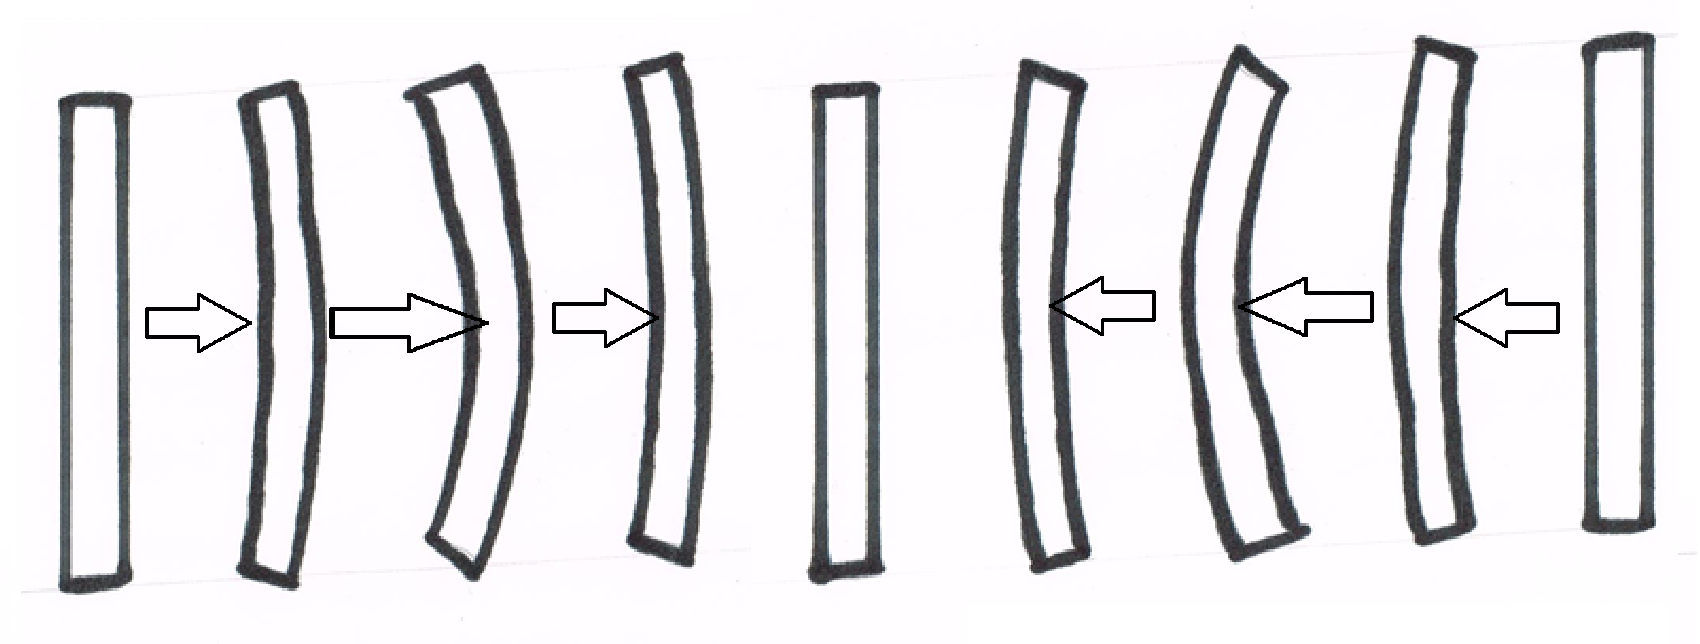
\includegraphics[width=5cm]{nsmr/img/supikasinndou.png}
  \caption{スピーカー振動版}
  \label{fig:spk}
\end{figure}
図\ref{fig:spk}のようにスピーカーの振動板が振動すれば、振動板の周りの空気は押されたり引かれたりします。これが空気の圧力の変化が伝わっていく現象です。\par
次に振動版によって押された空気がどうなったかをイメージしてみましょう。
\begin{figure}[H]
  \centering
  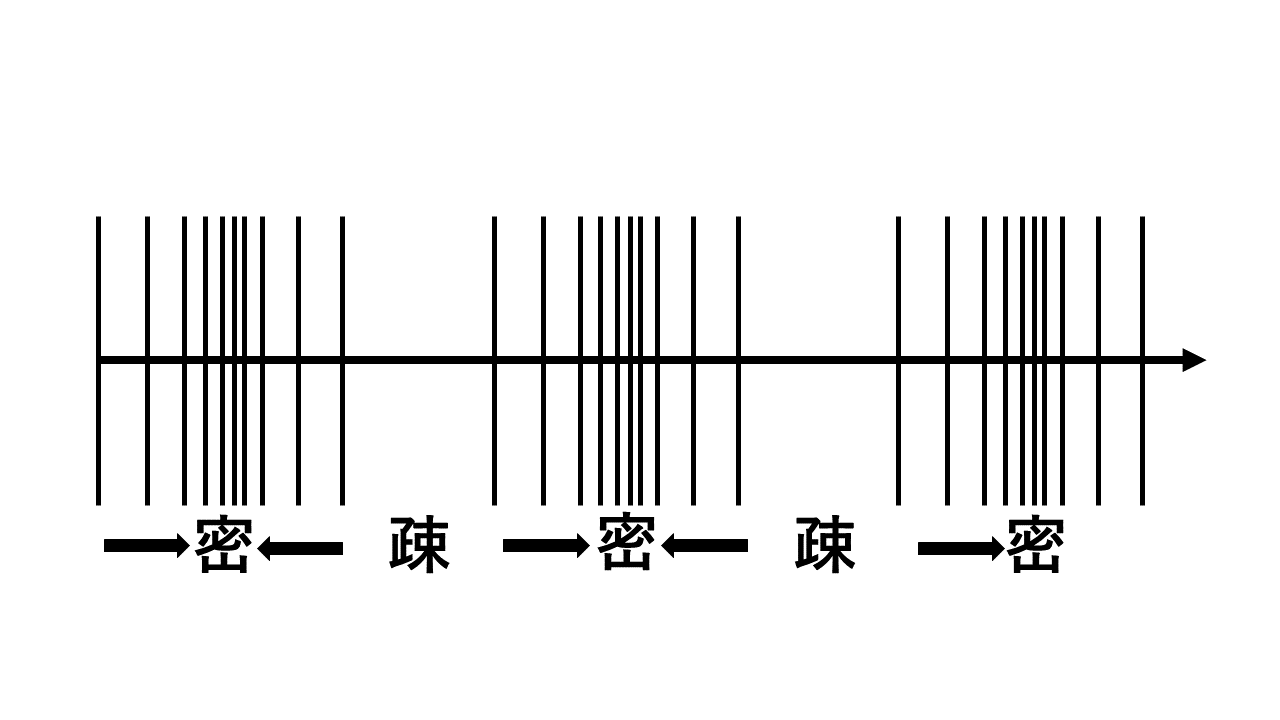
\includegraphics[width=5cm]{nsmr/img/slide4.png}
  \caption{空気の圧力変化}
  \label{fig:aturyoku}
\end{figure}
図\ref{fig:aturyoku}のように空気はばねのような振る舞いをし、空気には密な部分や疎な部分ができます。このように波の振動方向と進行方向が同じ波を縦波といいます。\par
縦波の他にも横波と呼ばれる波もあり、横波は進行方向と振動方向が垂直になる波のことです(図\ref{fig:yokonami})。また、縦波の表現を横波の表現にすることができ、逆に横波の表現を縦波の表現にすることもできます。縦波は空気分子の元の位置からのずれを変位として縦軸にとります。よって、空気の振動の変化を考えるには横波の表現のほうが分かりやすく適しています。
\begin{figure}[H]
  \centering
  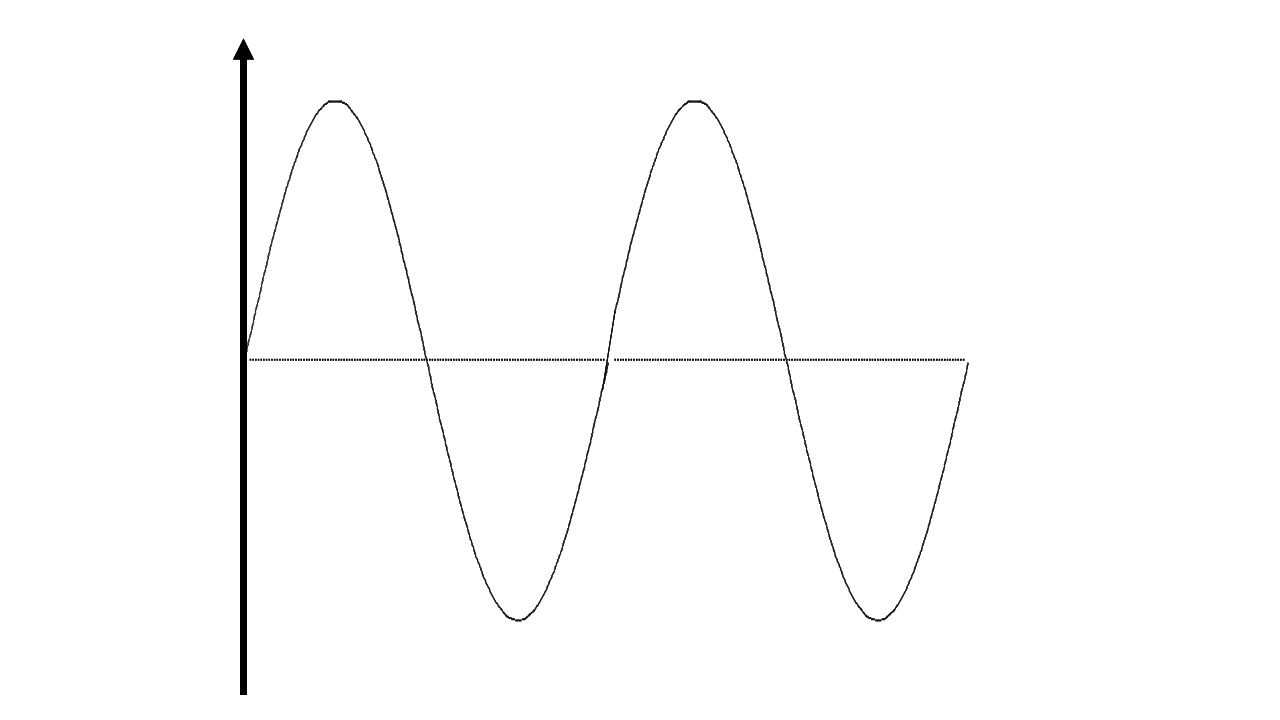
\includegraphics[width=5cm]{nsmr/img/slide16.png}
  \caption{横波}
  \label{fig:yokonami}
\end{figure}
横波を見てサイン波を思い浮かべる人も多いと思います。しかし、なかなか三角関数を日常生活で使うことはないと思うので忘れてしまった人もいますよね。次のセクションではサイン波ってどんな波だったかを復習します。



\subsection{波といえばサイン波}
サイン波は三角関数のひとつであるサイン関数で定義される波形です。この波形は周期的に山と谷が繰り返し現れ、最も基本的な波です(図\ref{fig:sinha})。
\begin{figure}[H]
  \centering
  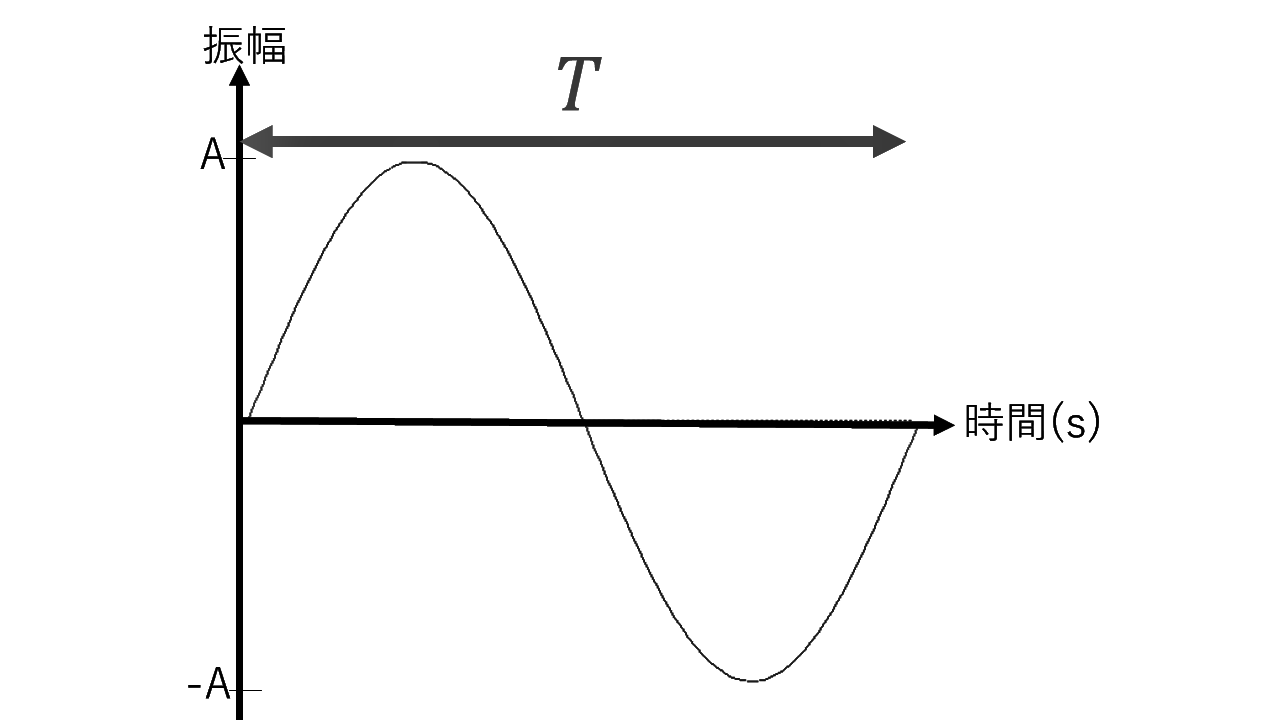
\includegraphics[width=5cm]{nsmr/img/slide15}
  \caption{サイン波}
  \label{fig:sinha}
\end{figure}
波を表すパラメータには振幅・周期があります。振幅は波の山(谷)の高さ、周期は波1つが波1つ分進むのにかかる時間を表します。音の場合は波の振幅は音の大きさ、周期は音の高さに対応しています。よく音の高さを表す時の単位として[Hz:ヘルツ]が使われますが、これは音の周波数の単位です。周波数とは1秒間で波形が何個現れるかを表すパラメータです。周期$T_0$と周波数$f_0$の関係は以下の式で表されます。
\begin{align}
  f_0=\frac{1}{T_0}
\end{align}
例えば、周期が$2\tani{s}$の波は$2\tani{s}$ごとに同じ波が繰り返し現れることを意味し、周期$2\tani{s}$の波であると言えますが、1秒間で$1/2$個(1波長の半分)が現れるので振動数$1/2\tani{Hz}$の波とも言えます。\par
また、振幅を$A$として、時刻$t$を変数とするサイン波は以下のように表せます。
\begin{align}
  u(t)=A\sin{(2\pi f_0 t)}
\end{align}
この式の$\sin{()}$の中身について、$f_0$と$t$の積は一周期を繰り返す回数を表していて、それにサイン関数の一周期$2\pi \tani*{rad}$をかけていることから、一周期$2\pi \tani*{rad}$を$f_0 t$回繰り返すという意味であることが分かります。
実際に先ほどの例で用いた周期$2\tani{s}$(振動数$1/2\tani{Hz}$)の波を振幅$1$としてグラフ化してみます。\par
上式の$f_0$を$f_0=\frac{1}{2}$とすると図\ref{fig:sintwo}のようになります。
\begin{figure}[H]
  \centering
  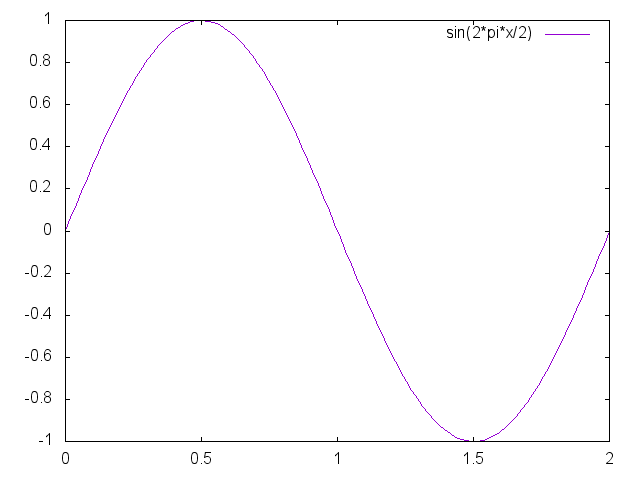
\includegraphics[width=5cm]{nsmr/img/sin05.png}
  \caption{周期$2\,\mathrm{s}$のサイン波}
  \label{fig:sintwo}
\end{figure}
図\ref{fig:sintwo}より、確かに一周期が$2\tani{s}$であり、$1\tani{s}$で一周期の波の半分が現れることが確認できました。
%
\newpage
\section{音の分析にチャレンジ!}
\subsection{周波数特性}
波を表す方法として、縦軸を振幅、横軸を時間にするやり方の他にも、縦軸を振幅、横軸を周波数にする方法もあります。後者の方法で表すグラフを周波数特性といいます。図\ref{fig:sintwo}の振幅-時間グラフの周波数特性は図\ref{fig:shuuhasuutoku}になります。
\begin{figure}[H]
  \centering
  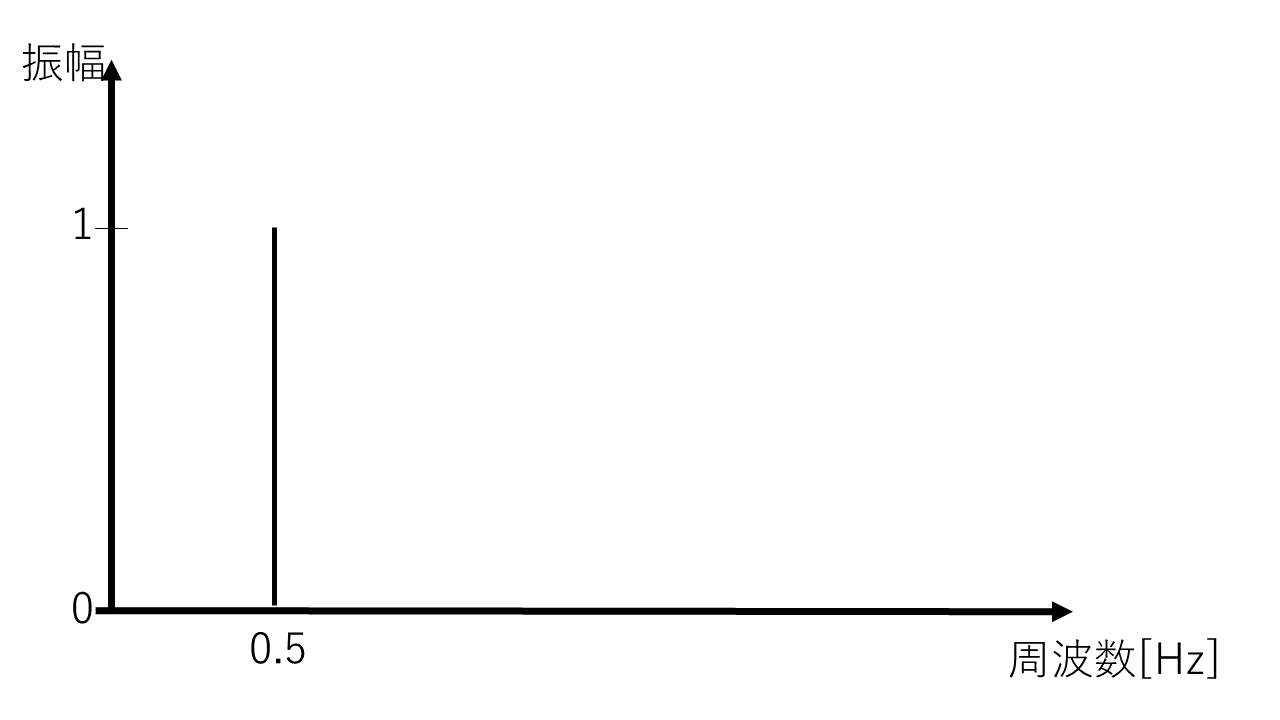
\includegraphics[width=8cm]{nsmr/img/slide17.PNG}
  \caption{周波数特性}
  \label{fig:shuuhasuutoku}
\end{figure}
波を表すのに振幅-時間グラフを用いる利点は、直感的に波を捉えることができる点です。横軸を時間にすることで波の時間発展による変化を捉えやすくなります。\par
周波数特性のグラフを用いる利点は、波を構成している波の周波数が一目で分かるという点です。
これまでの議論では最も単純な波であるサイン波1つのみを考えてきたので、周波数特性のグラフを使う恩恵をあまり感じることができませんが、いくつかの周波数成分を持つ波を解析するときには振幅-時間グラフではどの振動数の波が含まれているかが分かり難いです。\par
これまで考えてきた1つの周波数成分のみで構成される音を純音、いくつかの周波数成分を持つ波のことを複合音といいます。大切なのは、すべて複合音は純音の重ね合わせで表現できるということです。

%
\newpage
\subsection{フーリエ級数展開}
複合音が純音の重ね合わせで書けるということを言い換えると、複雑な波でも周期的であれば周期的で単純な波であるサイン波やコサイン波の和で書けるということになります。\par
複雑な周期関数がサイン関数とコサイン関数の和で表わすことをフーリエ級数展開といいます。

\begin{itembox}[l]{フーリエ級数展開}
  $f(x)$を周期$2\pi$の周期関数とすると、$f(x)$は
  \begin{align}
    f(x) =\sum_{n=0}^{\infty}(a_n \cos(nx)+b_n \sin(nx))
  \end{align}
    と無限級数に展開できる。また、$a_0,a_n,b_n$は以下の式で表せる。$(n\geq1)$
  \begin{align}
    a_0 &= \frac{1}{2\pi}\int_{-\pi}^{\pi} f(x) dx,\\
    a_n &= \frac{1}{\pi}\int_{-\pi}^{\pi} f(x) \cos(nx) dx,\\
    b_n &= \frac{1}{\pi}\int_{-\pi}^{\pi} f(x) \sin(nx) dx.
  \end{align}
\end{itembox}

ここからは具体的な関数を考えてみましょう。
ここでは矩形波をフーリエ級数展開してみます。矩形波とは半周期ごとに一定値のハイと
ロー(ハイの符号を逆にしたもの)を繰り返す波のことです。矩形波は図\ref{fig:kukeihae}のような形をしています。
\begin{figure}[H]
  \centering
  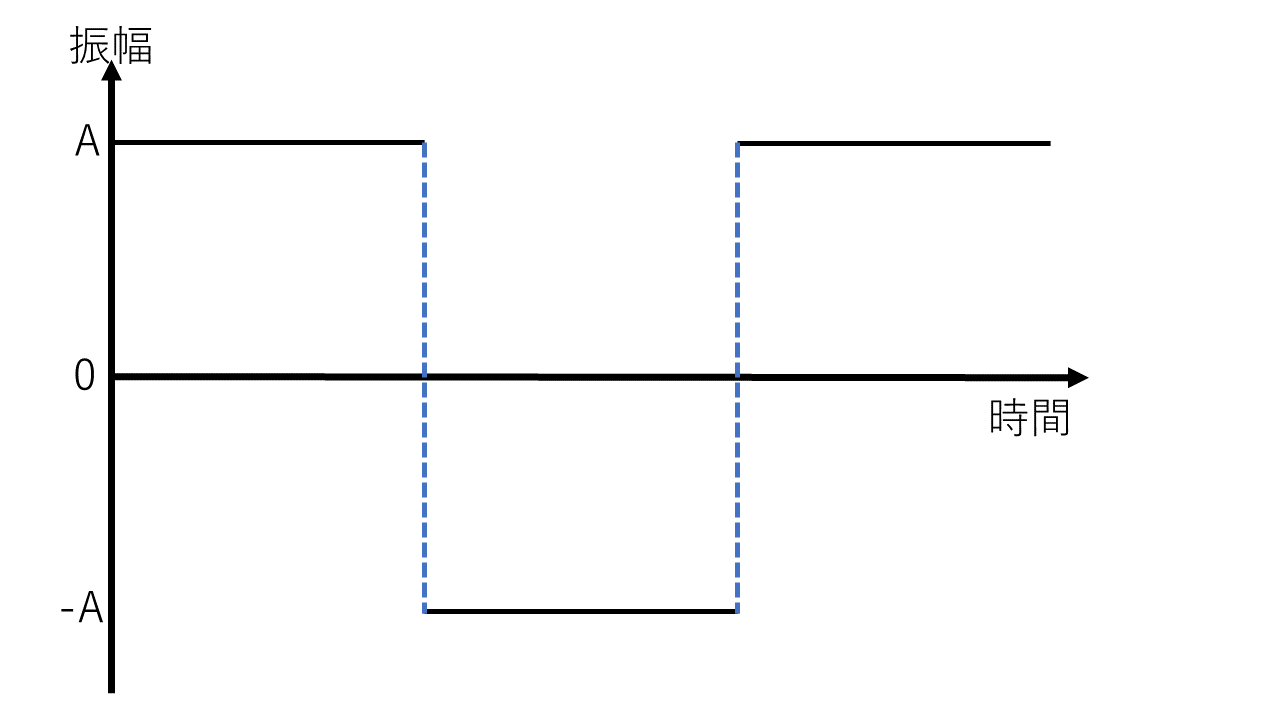
\includegraphics[width=5cm]{nsmr/img/slide5.png}
  \caption{矩形波形の形}
  \label{fig:kukeihae}
\end{figure}
これを関数として表現すると
\begin{align}
  f(x)=
    \begin{cases}
      1 &\quad (0<x<\pi)\\
      -1 &\quad (-\pi<x<0)
    \end{cases}
\end{align}

ここで、$f(x)$は奇数関数、$\cos(nx)$は偶関数なので $f(x)\cos(nx)$ は奇関数となり、
$-\pi$から$\pi$まで積分すると値が0になるので$a_n$は$0$になります。\par
また、$f(x)\sin(nx)$は偶関数なので$-\pi$から$\pi$まで積分するのは、$0$から$\pi$まで積分して二倍にすることと同値です。つまり、$b_n=\frac{2}{\pi}\int_{0}^{\pi} f(x) \sin(nx) dx$を求めればよいです。\par
以上より
\begin{align}
  f(x) &= \sum_{n=0}^{\infty} b_n \sin(nx) \label{siki:furie1}\\
  b_n &= \frac{2}{\pi}\int_{0}^{\pi}  f(x) \sin(nx) dx \label{siki:furie2}
\end{align}
式(\ref{siki:furie1}),式(\ref{siki:furie2})を解けば矩形波の関数$f(x)$をフーリエ級数展開できます。
\begin{align}
  b_n &=\frac{2}{\pi}\int_{0}^{\pi}  f(x) \sin(nx) dx \nonumber\\
  &=\frac{2}{\pi}\int_{0}^{\pi} \sin(nx) dx \nonumber\\
  &=\frac{2}{\pi}\qty[-\frac{1}{n}\cos(nx)]_{0}^{\pi} \nonumber\\
  &=-\frac{2}{n\pi}(\cos(n\pi)-1) \nonumber\\
  &=
  % \begin{cases}
  %   -\dfrac{2}{n\pi}(-1-1) &\quad (n=1,3,5...)\\
  %   -\dfrac{2}{n\pi}(1-1) &\quad (n=2,4,6...)\nonumber\\
  % \end{cases}\\
  \begin{dcases}
    -\dfrac{2}{n\pi}(-1-1) &\quad (n=1,3,5...)\\
    -\dfrac{2}{n\pi}(1-1) &\quad (n=2,4,6...)\nonumber\\
  \end{dcases}\\
  &=
  % \begin{cases}
  %   \dfrac{4}{n\pi} &\quad (n=1,3,5...)\\
  %   \vphantom{\dfrac11} 0 &\quad (n=2,4,6...)
  % \end{cases}
  \begin{dcases}
    \dfrac{4}{n\pi} &\quad (n=1,3,5...)\\
    \vphantom{\dfrac11} 0 &\quad (n=2,4,6...)\label{siki:112418}
  \end{dcases}
\end{align}
式(\ref{siki:112418})を式(\ref{siki:furie1})に代入して計算すると
\begin{align}
  f(x) &= \sum_{n=1,3,5...}\frac{4}{n\pi}\sin(nx) \nonumber\\
  &= \sum_{m=0}^{\infty}\frac{4}{(2m+1)\pi}\sin((2m+1)x)\nonumber\\
  &= \frac{4}{\pi} \qty\Big(\sin x +\frac{1}{3}\sin 3x+\frac{1}{5}\sin 5x+\cdots)
\end{align}
以上より、矩形波を周期関数$f(x)$に見立てたとき$f(x)$は
\begin{align}
  f(x)&= \frac{4}{\pi} \qty\Big(\sin x +\frac{1}{3}\sin 3x+\frac{1}{5}\sin 5x+\cdots)
  \label{fig:sinnowa}
\end{align}
というようにサイン関数の和で書けることがわかりました。\par
ここで再び、この周期関数を矩形波として扱うために、
周波数を$f_0$、時間を$t$として$x=2\pi f_0 t$とします。式(\ref{fig:sinnowa})に代入すると
\begin{align}
f(t) &= \frac{4}{\pi} \qty\Big(\sin( 2\pi f_0 t) + \frac{1}{3}\sin (3\times 2\pi f_0 t)+\frac{1}{5}\sin (5\times2\pi f_0 t)+\cdots) \nonumber\\
&=\frac{4}{\pi} \qty\Big(\sin( 2\pi f_0 t) +\frac{1}{3}\sin (2\pi (3f_0) t)+\frac{1}{5}\sin (2\pi (5f_0) t)+\cdots) \label{fig:sinwakaru}
\end{align}
式(\ref{fig:sinwakaru})からわかることはいろいろな周期・振幅のサイン波が合成されており、
例えば第二項目のサイン波の周波数は第一項目のサイン波の周波数の3倍であるが、
振幅は$1/3$倍になっていることです。つまり、$n$を自然数とし、
第$n$項目のサイン波は第一項目のサイン波と比べると周波数は$2n-1$倍、
振幅は$1/(2n-1)$倍のサイン波であることがわかります。\par
では、具体的に1周期$2\tani{ms}$の矩形波を作ってみましょう。\par
今回計算に使うプログラミング言語はFortranです。$n$を入力し、サイン波を第$n$項目まで足し合わせるというプログラミングです。以下、ソースコードを記載します。

% \begin{screen}
% \begin{verbatim}
%       implicitnone\\
%       real*8 pi,y,t,A\\
%       integer n,m,x\\
%       open(10,file='kukeiha.dat',status='unknown')\\
%       pi=4.0*atan(1.0)\\
%       write(*,*)"nを入力"\\
%       read(*,*) n !2n+1倍音まで足し合わせるためのnを入力\\
%       \\
%       do x=0,4000\\
%         y=0.d0 !yの初期化\\
%         t=x/1000000.d0 !時間を0msから4msまで0.001ms刻みで増やすため\\
% \\
%       do m=1,n\\
%         A=2.d0*m-1.d0\\
%         y=(4.d0/pi)*(1.d0/A)*sin(A*t*2.d0*pi/0.002)+y\\
%       enddo\\
% \\
%       write(10,*)t,y\\ 
% \\
%       enddo \\
%       close(10)\\
%       stop\\
%       end
% \end{verbatim}
% \end{screen}

\begin{screen}
\begin{verbatim}
    implicitnone
    real*8 pi, y, t, A
    integer n, m, x
    open(10, file='kukeiha.dat', status='unknown')
    pi = 4.0*atan(1.0)
    write(*,*) "nを入力"
    read(*,*) n !2n+1倍音まで足し合わせるためのnを入力

    do x = 0, 400
      y = 0.d0 !yの初期化
      t = x/100000.d0 !時間を0msから4msまで0.01ms刻みで増やすため

      do m = 1, n
        A = 2.d0*m - 1.d0
        y = (4.d0/pi)*(1.d0/A)*sin(A*t*2.d0*pi/0.002) + y
      enddo

      write(10,*) t, y

    enddo
    close(10)
    stop
    end
\end{verbatim}
\end{screen}

\newpage
図\ref{fig:nhikaku}に$n=1,2,3,10$項目までサイン波を足し合わせたグラフをそれぞれ記載します。\par
足し合わせる項数が多いほど矩形波に近づくことがわかります。
\begin{figure}[H]
  \centering
  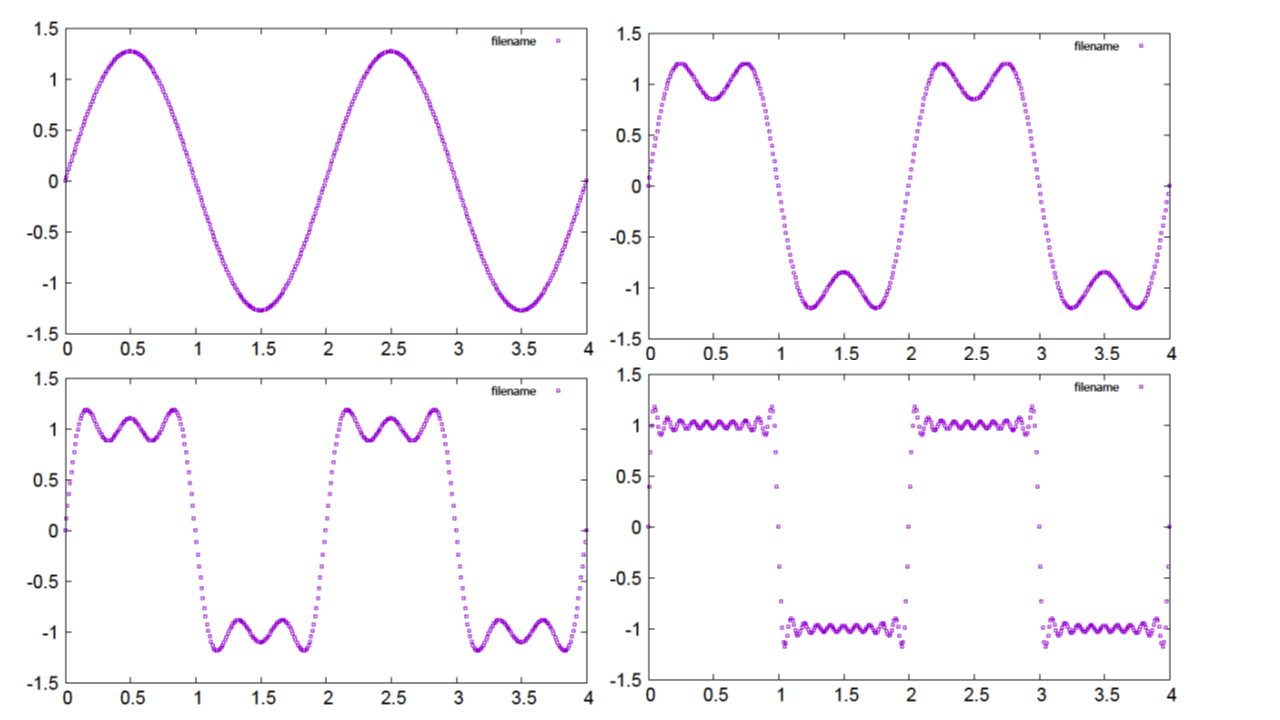
\includegraphics[width=10cm]{nsmr/img/n==12310.png}
  \caption{n=1,2,3,10項目までサイン波を足し合わせた結果(左上:$n=1$,右上:$n=2$,左下:$n=3$,右下:$n=10$)}
  \label{fig:nhikaku}
\end{figure}
次に図\ref{fig:ngath}に$n=1000$項目までサイン波を足し合わせたグラフを記載します。\par
1000項目まで足し合わせると、理想的な矩形波になっていることがわかります。

\begin{figure}[H]
  \centering
  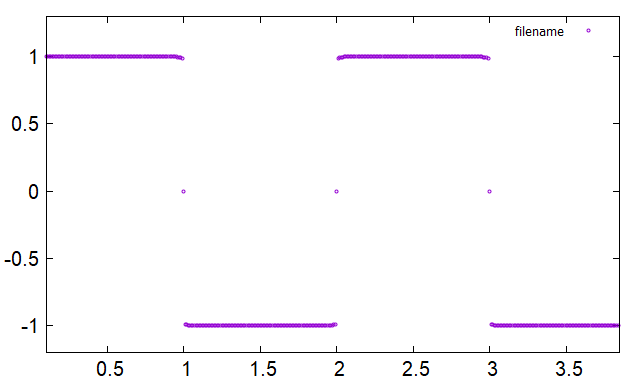
\includegraphics[width=5cm]{nsmr/img/n==1000.png}
  \caption{n=1000項目までサイン波を足し合わせた結果}
  \label{fig:ngath}
\end{figure}
周期$2\tani{ms}$の矩形波の周波数特性で最も大きな割合を占めるのは
周波数$f_0=1/0.002=500\tani{Hz}$でありこのサイン波を基本振動というと、
残りの合成されているサイン波の周波数は基本振動の周波数$f_0$の奇数倍のものだけであり、
振幅は基本振動の振幅の奇数分の1倍の大きさになっています。\par
\newpage
以上の結果を矩形波の周波数特性としてグラフにすると図\ref{fig:kukeihashuuha}になります。
\begin{figure}[H]
  \centering
  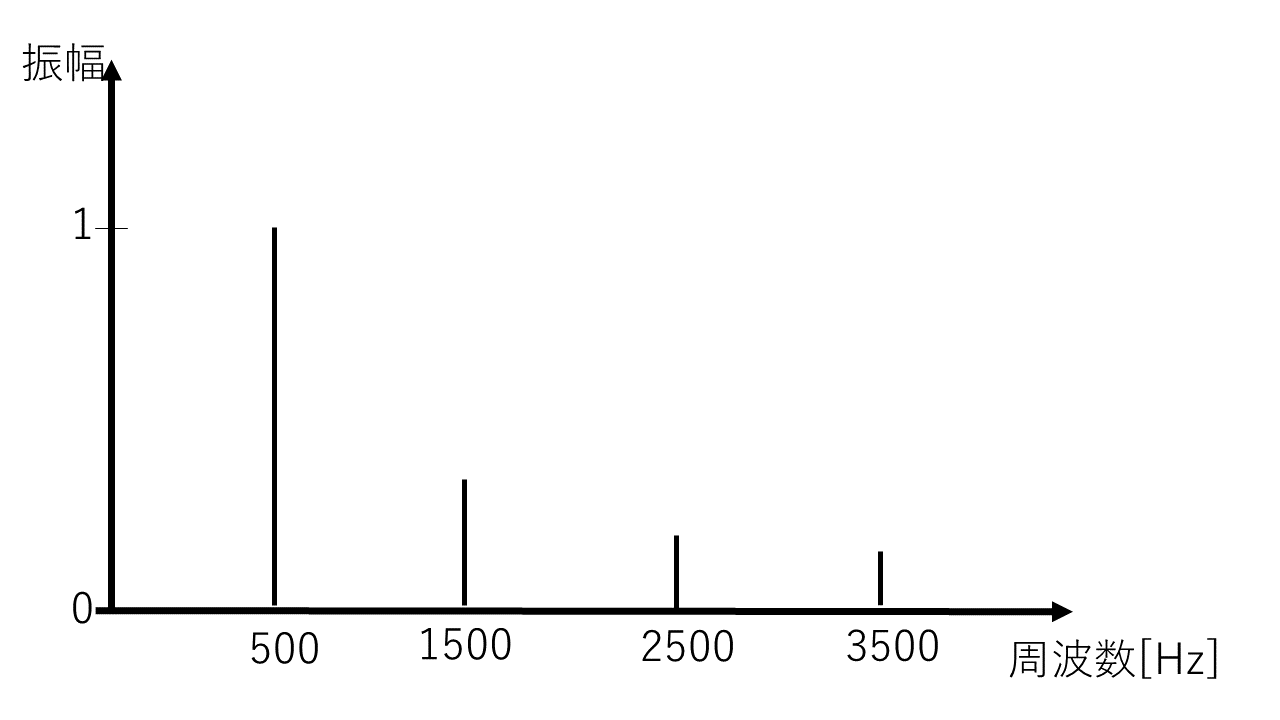
\includegraphics[width=5cm]{nsmr/img/slide6.png}
  \caption{矩形波の周波数特性}
  \label{fig:kukeihashuuha}
\end{figure}


% - - - - - - - - - - - - - - - - - - -
\if0
\subsection{周波数分析の方法(フィルタ編)}
周波数分析を行う方法として使われるのがフィルタです。フィルタは特定の周波数成分の波だけ通して、それ以外を通さないというものです。\par
フィルタにはいくつかの種類があり、低域の周波数成分のみを通過させる低域通過フィルタ、逆に高域の周波数成分のみを通過させる高域通過フィルタ、特定の帯域の周波数成分のみを通過させる帯域通貨フィルタ、特定の周波数成分を減衰させる帯域阻止フィルタなどがあります。

\begin{figure}[H]
  \begin{minipage}{0.33\hsize}
  \begin{center}
  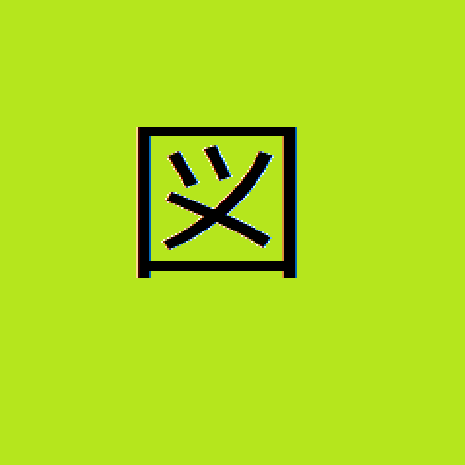
\includegraphics[width=3cm]{nsmr/img/zu.png}
	\end{center}
  \caption{低域}
\end{minipage}
 \begin{minipage}{0.33\hsize}
  \begin{center}	
 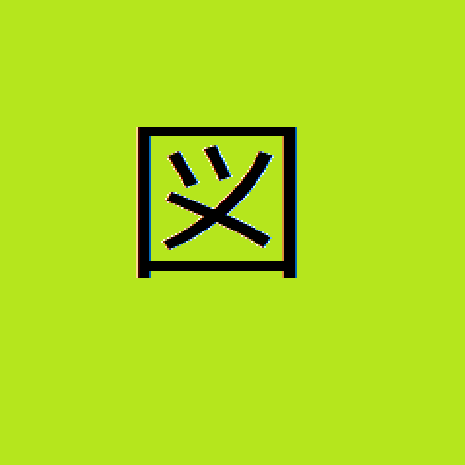
\includegraphics[width=3cm]{nsmr/img/zu.png}
 \end{center}  
\caption{高域}
\end{minipage}
\end{figure}
\begin{figure}[H]
  \begin{minipage}{0.33\hsize}
  \begin{center}
  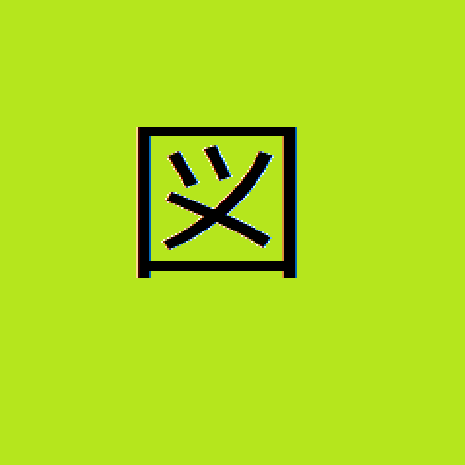
\includegraphics[width=3cm]{nsmr/img/zu.png}
	\end{center}
  \caption{通過}
\end{minipage}
 \begin{minipage}{0.33\hsize}
  \begin{center}	
 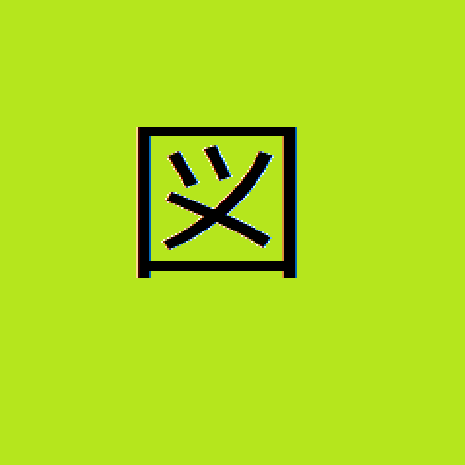
\includegraphics[width=3cm]{nsmr/img/zu.png}
 \end{center}  
\caption{阻止}
\end{minipage}
\end{figure}
\fi
% - - - - - - - - - - - - - - - - - - -

%
\subsection{フーリエ変換で周波数分析!}
これまでのお話で純音以外の音(複合音)も純音を足し合わせることで表すことができるということを述べてきましたが、具体的に複合音の中に含まれる純音の周波数・振幅を解析することを周波数分析といいます。\par
図\ref{fig:furie}のように窓を使い波形を区切りそのなかに含まれる波の周波数特性を求める方法がフーリエ変換です。フーリエ変換では複合音は大小様々な波長の波が合成されており、その波長の波がどれぐらいの振幅でもって合成されているのかを分析します。窓の大きさを$\Delta t$とすると、波形に当てはめることのできるサイン波の最小周波数$\Delta f$は以下のように表せます。
\begin{align}
  \Delta f=\frac{1}{\Delta t}
\end{align}
当てはめることのできる最小のサイン波の周波数が制約されるのは、当てはめることのできる最大の周期のサイン波が制約されるからです。窓の大きさに対して、当てはめるサイン波の周期が大きい場合というのは窓に当てはめるサイン波の1周期が窓1つに入りきらないことを意味します。よって、入りきらないということは最大の周期のサイン波を含むことができないことになるので制約を受けます。\par
周波数特性の周波数分布は$\Delta f$の整数倍の値のみ持ちます。また、窓の大きさ$\Delta t$が大きいと周波数分析の精度が上がります。なぜならば、窓の大きさが大きいほど含まれているサイン波の最小周波数$\Delta f$が小さくなるからです。
\begin{figure}[H]
  \centering
  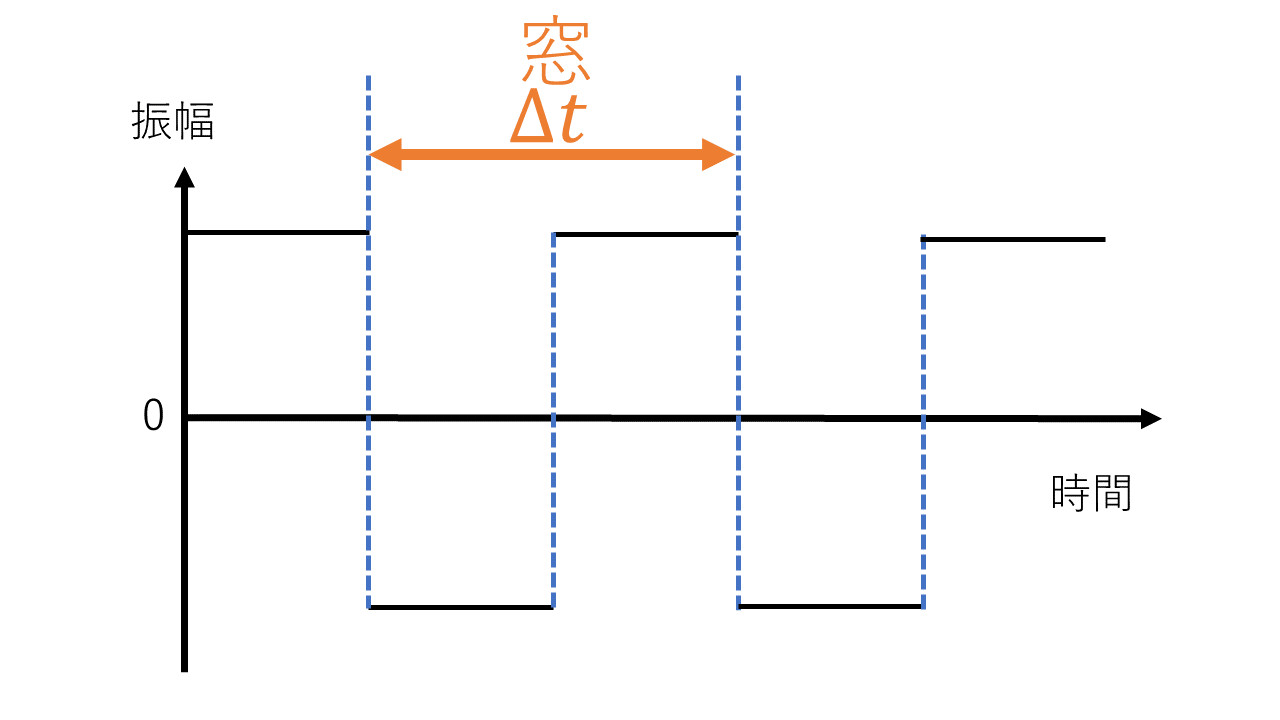
\includegraphics[width=5cm]{nsmr/img/slide11.png}
  \caption{フーリエ変換}
  \label{fig:furie}
\end{figure}
では、実際に波形をフーリエ変換して周波数特性を求めてみましょう。
先ほど、フーリエ級数展開で矩形波の周波数特性を求めたので、このソフトを使って矩形波の周波数特性を求めて、結果が一致するかどうかを確かめてみます。\par
まずは波形を作るところから始めます。今回はインターネットでダウンロードできるフリーソフト「WaveGene」	を使います。「WaveGene」は\url{<http://efu.jp.net/soft/wg/wg.html>}からダウンロードできます。\par
図\ref{fig:wavegene}に「WaveGene」で作った周期$2\tani{ms}$の矩形波を記載します。
\begin{figure}[H]
  \centering
  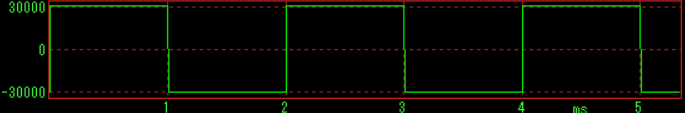
\includegraphics[width=10cm]{nsmr/img/wavegine.png}
  \caption{Wavegeneで作った矩形波}
  \label{fig:wavegene}
\end{figure}
この波形を、またまたフリーソフト「WaveSpectra」を使い解析します。「WaveSpectra」は
\url{<http://efu.jp.net/soft/ws/ws.html>}からダウンロードできます。「WaveSpectra」は波をフーリエ変換し、周波数特性を出してくれます。\par
図\ref{fig:wavespe}に矩形波を「WaveSpectra」で周波数解析した結果を記載します。
\begin{figure}[H]
  \centering
  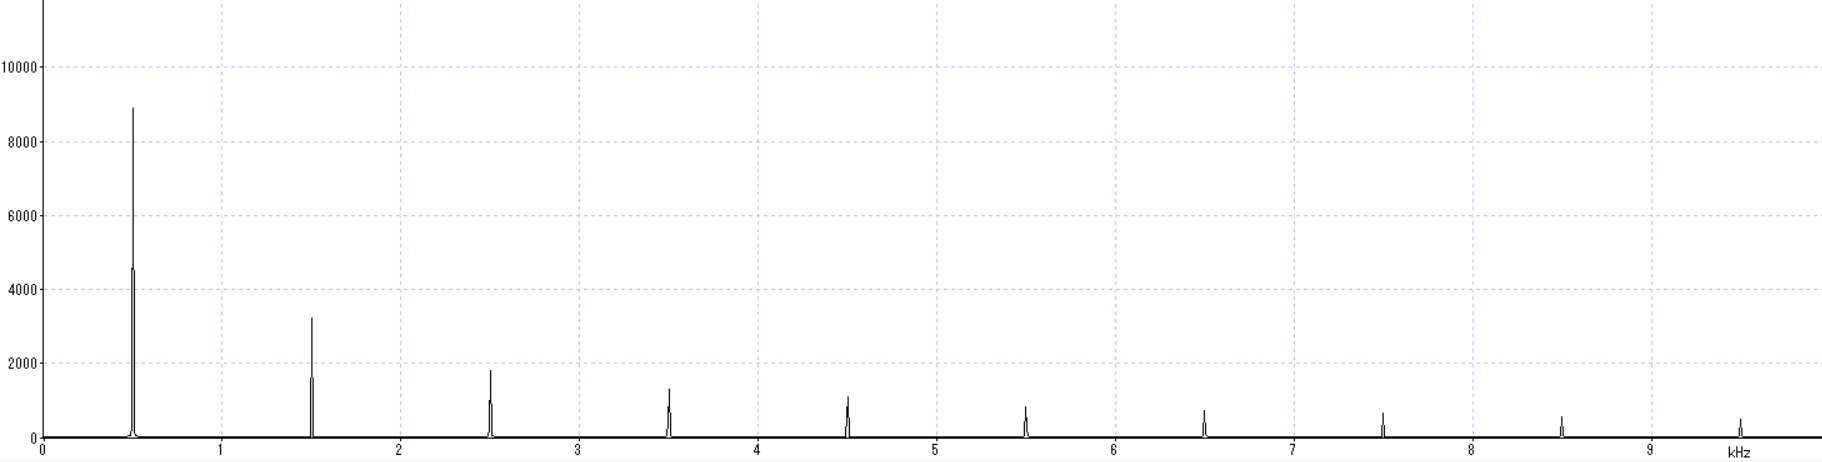
\includegraphics[width=10cm]{nsmr/img/kukeihawav2.png}
  \caption{WaveSpectraで解析した矩形波の周波数特性}
  \label{fig:wavespe}
\end{figure}
図\ref{fig:wavespe}と級数展開の結果を比べると結果は一致することが分かります。

%
\subsection{スペクトログラム}
これまでは時間変化によって音(周波数)が変わらない場合の周波数特性を求めるために、窓で波形を区切ってフーリエ変換を用い周波数特性を求めていましたが、実際の音は時間発展によって変化するものもあるので、一般的には音の周波数特性を調べる場合は時間ごとの周波数特性を求める必要があります。\par
方法としてはこれまでと同じく窓の中の音をフーリエ変換しつつ、その窓を時間変化に応じて少しずつずらしていくという手法です。窓を少しずつずらすことで周波数分析を時間的に連続して行うことができます。\par
以上の手法を用いた結果得られる周波数特性を表すグラフをスペクトログラムといいます。スペクトログラムは横軸を時間、縦軸を周波数として、色の濃さでその周波数の音の強さ(大きさ)を表します。
図\ref{fig:spemae}→図\ref{fig:spetyuu}→図\ref{fig:spego}の順に進み最後の図\ref{fig:spego}がスペクトグラムです。
\begin{figure}[H]
  %
  \begin{minipage}{0.32\hsize}
    \begin{center}
      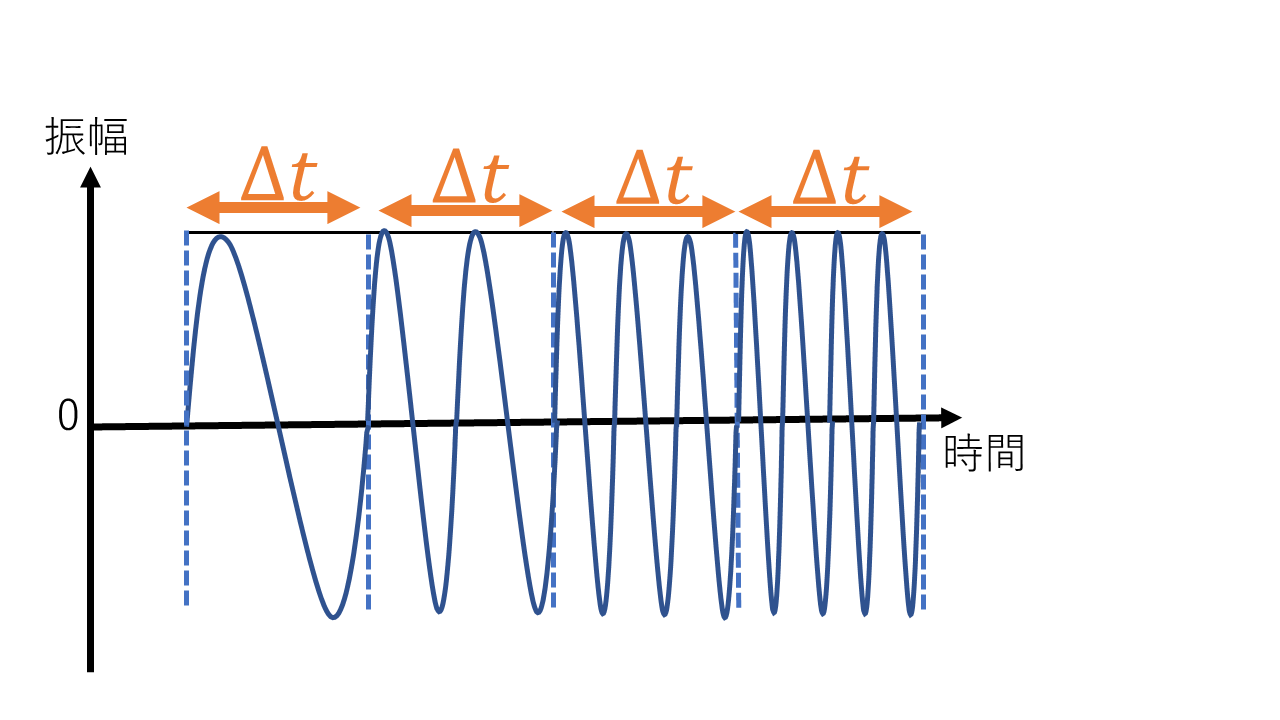
\includegraphics[width=4cm]{nsmr/img/slide12.png}
    \end{center}
    \caption{窓をずらす}
    \label{fig:spemae}
  \end{minipage}
  %
  \begin{minipage}{0.33\hsize}
    \begin{center}	
      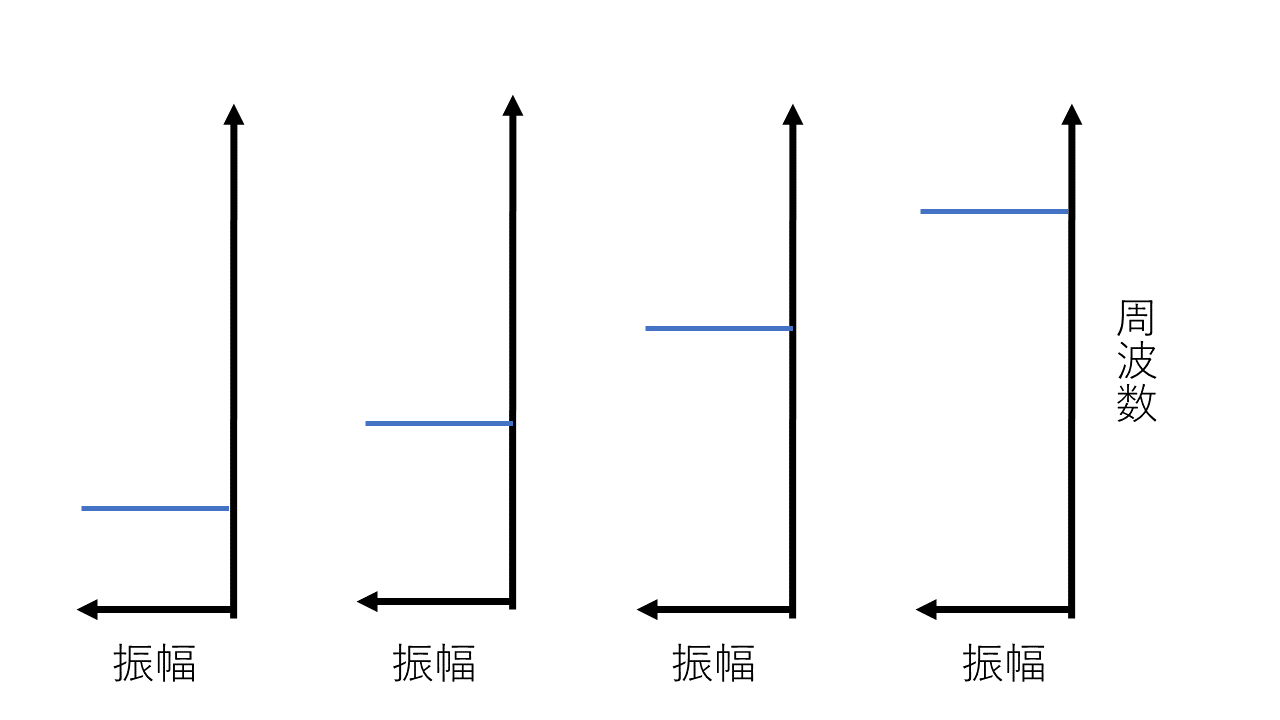
\includegraphics[width=4cm]{nsmr/img/slide13.png}
    \end{center}  
    \caption{ずらした窓でフーリエ変換}
    \label{fig:spetyuu}
  \end{minipage}
  %
  \begin{minipage}{0.33\hsize}
    \begin{center}
      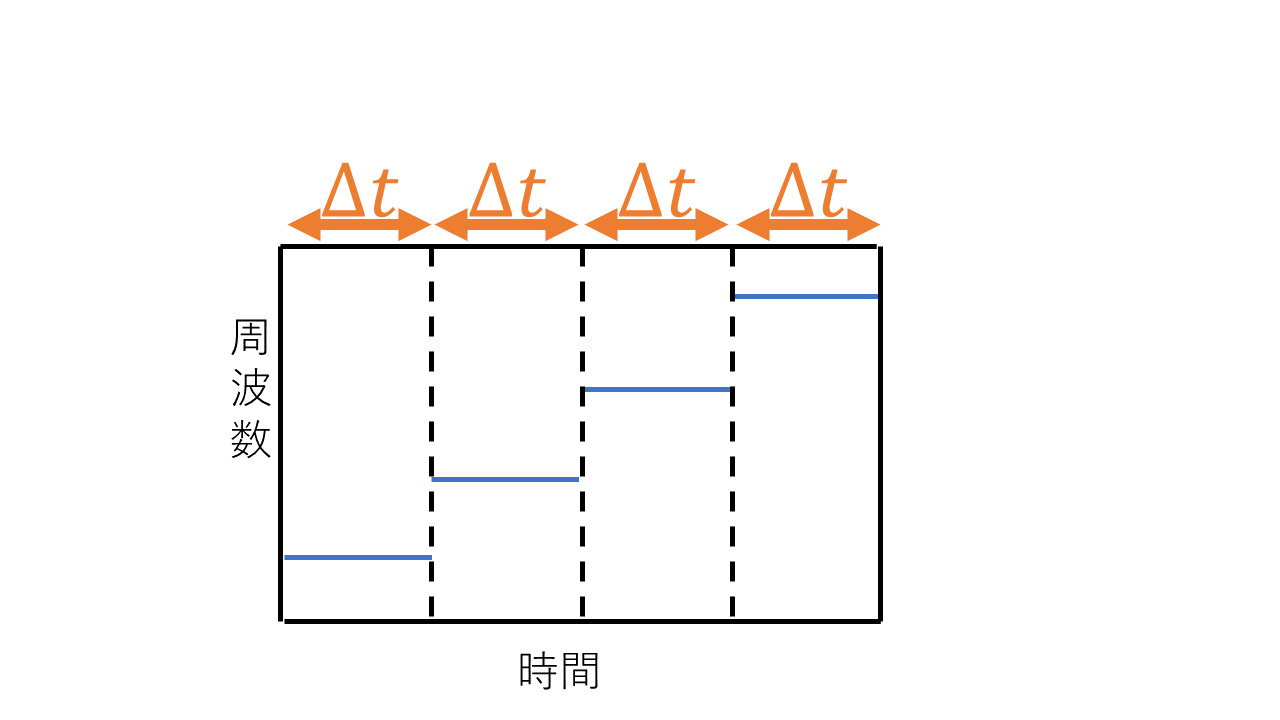
\includegraphics[width=4cm]{nsmr/img/slide14.png}
    \end{center}
    \caption{スペクトログラム}
    \label{fig:spego}
  \end{minipage}
  %
\end{figure}

%
\subsection{不確定性原理}
周波数分析の精度は窓の大きさによって決まります。時間に応じて音が変化する場合は、時間を区切ることと周波数を区切ることを別々に行い、区切られた中の音の周波数特性を調べます。\par
時間を区切る間隔を小さくすると、より時間の変化に対して観測で得られるスペクトグラムが敏感になるので、時間変化を詳細に調べることができます。同様に周波数を区切る間隔を小さくすると、より周波数特性を詳細に調べることができます。
以上より時間を区切る間隔は時間分解能、周波数を区切る間隔は周波数分解能を表すことがわかります。\par
\newpage
時間分解能を$\Delta t$、周波数分解能を$\Delta f$とすると、この二つの関係は以下のようになります。
\begin{align}
  \Delta f \propto \frac{1}{\Delta t}
\end{align}
上式の意味は時間分解能と周波数分解能が反比例の関係であることです。この関係から時間分解能と周波数分解能のどちらも低い値にすることができないということがわかります。仮に時間変化を詳細に調べようとすると時間分解能を低くするので、周波数分解能が高くなり、周波数特性の周波数部分が曖昧になります。同様に周波数特性を詳細に調べようとすると、周波数特性の時間変化の部分が曖昧になります。\par
このように片方を小さくすると片方が大きくなり、二つを同時に小さくできないことを不確定性原理といいます。\par
時間分解能を小さくしたスペクトログラムを広帯域スペクトログラムといい、周波数分解能を小さくしたスペクトログラムを狭帯域スペクトログラムといいます。前者は周波数分解能が大きくなり、帯域通過フィルタの帯域幅を大きくして周波数分析を行うこと同じなので「広帯域スペクトログラム」、反対に後者は帯域通過フィルタの帯域幅を小さくして周波数分析を行うので「狭帯域スペクトログラム」という名前が付けられています。

%
\subsection{スペクトグラムを見てみよう}
では、実際にスペクトグラムを見てみましょう。\par
今回は「Audacity」というオープンソースのオーディオソフトウェアを使ってスペクトグラムを見ます。\par
「Audacity」は\url{<https://www.audacityteam.org/>}からダウンロードできます。\par
Audacityを使うと、音波を縦軸:振幅、横軸:時間とした横波の図を表示させたり、その横波の周波数特性やスペクトグラムを分析することができます。\par
まず最初に同じ音源に対して、先ほど紹介した広帯域スペクトグラムと狭帯域スペクトグラムの二種類で分析してみます。周期$2\tani{ms}$の矩形波の広帯域スペクトグラムと狭帯域スペクトグラムは
図\ref{fig:sema}のようになります。(上が広帯域スペクトグラム、下が狭帯域スペクトグラム)

\begin{figure}[H]
  % \begin{minipage}{0.33\hsize}
    \begin{center}
      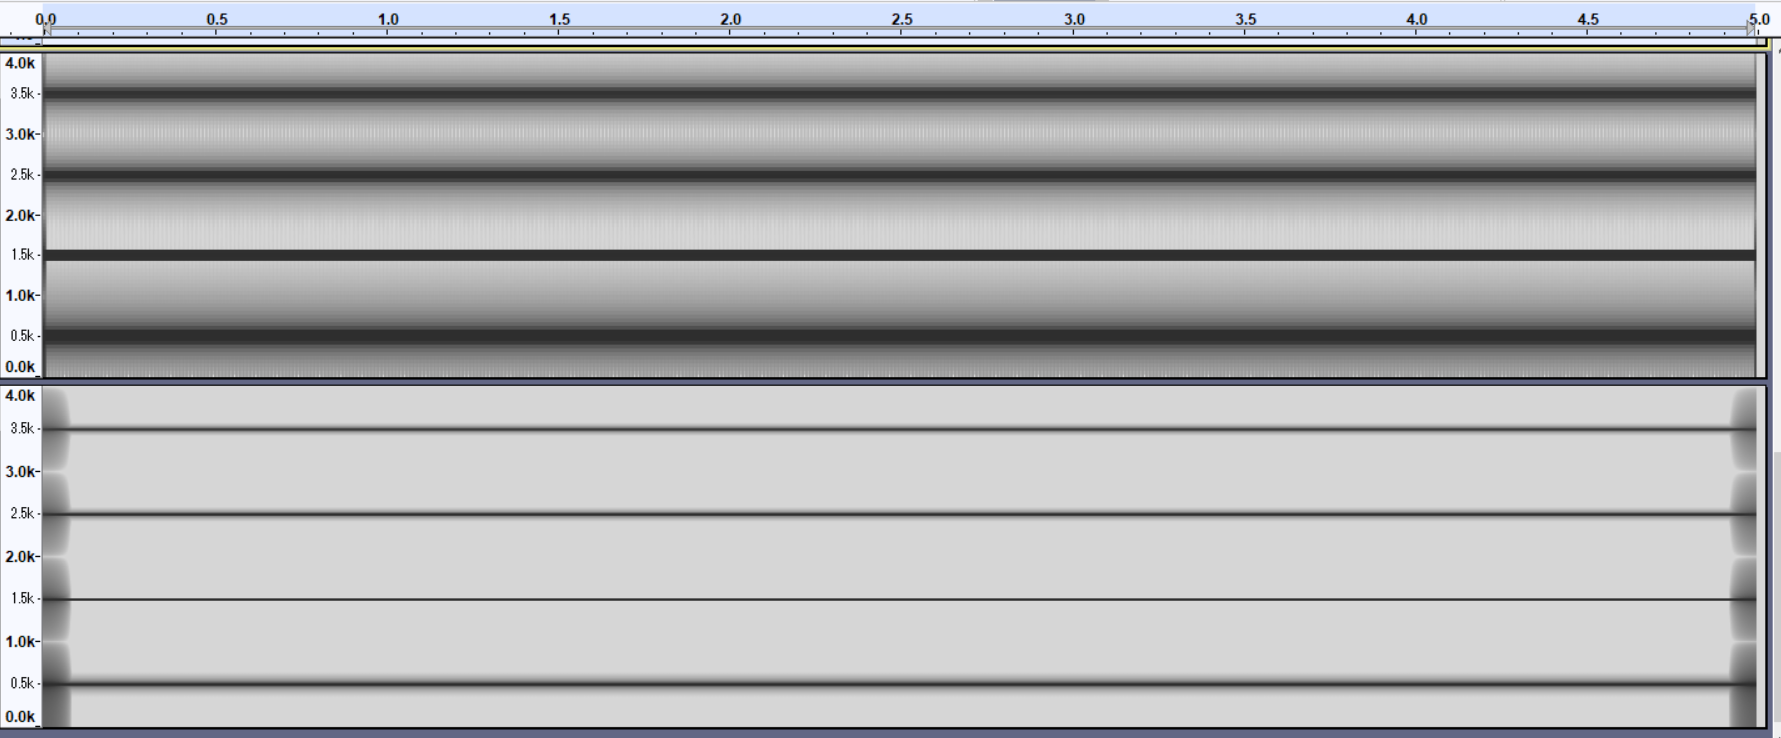
\includegraphics[width=10cm]{nsmr/img/timekukeiha.png}
    \end{center}
    \caption{矩形波の広帯域スペクトグラムと狭帯域スペクトグラム}
    \label{fig:sema}
  % \end{minipage}
\end{figure}
図\ref{fig:sema}より、広帯域スペクトグラムは周波数特性に広がりがあり、狭帯域スペクトグラムは周波数特性に広がりがありません。これは狭帯域スペクトグラムの方が周波数分解能が高いからです。よって、狭帯域スペクトグラムは周波数特性を分析するのに向いているということがわかります。また、周期$2\tani{ms}$の矩形波の周波数特性が確かに、これまで確認してきたような数値になっていることもわかります。
%%
次は時間発展により周波数が変わる音波のスペクトグラムを見てみましょう。\par
図\ref{fig:kukeisema}は「ブツリ」と言ったのを録音したものを周波数分析した結果で、上が広帯域スペクトグラムで下が狭帯域スペクトグラムです。

\begin{figure}[H]
  % \begin{minipage}{0.33\hsize}
    \begin{center}
      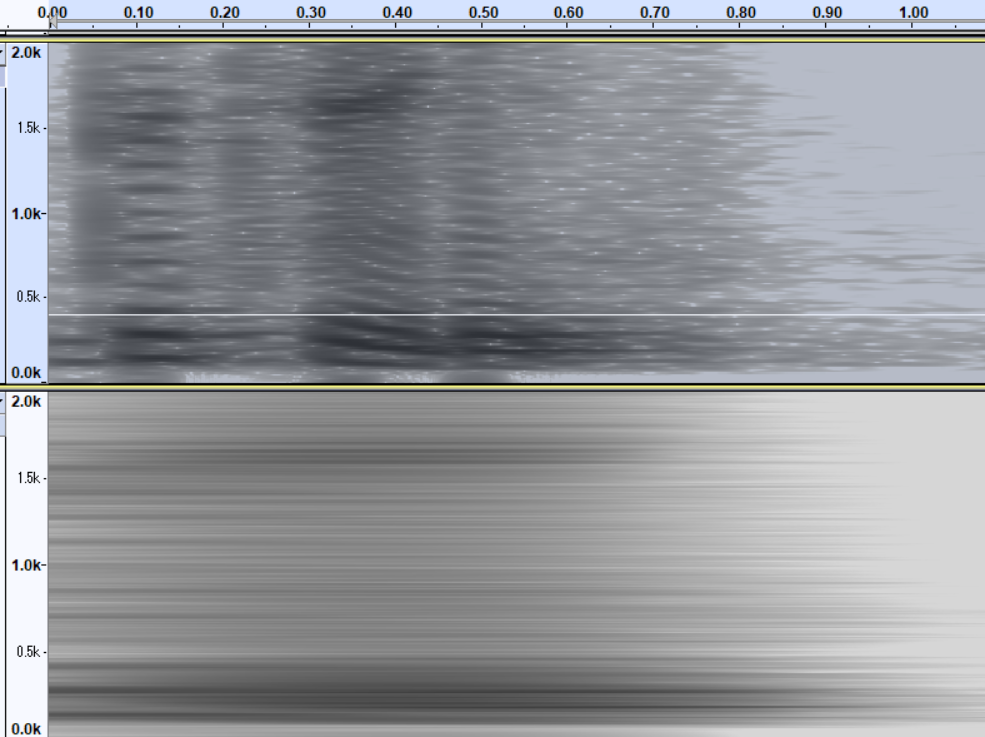
\includegraphics[width=8cm]{nsmr/img/saybuturi.png}
    \end{center}
    \caption{「ブツリ」という音声の広帯域スペクトグラムと狭帯域スペクトグラム}
    \label{fig:kukeisema}
  % \end{minipage}
\end{figure}

%
\subsection{言語の分析をしてみよう}
耳から得る情報の1つとして言語があります。日本語は50音で言葉を形成しますよね。\par
「あ」の音は誰が聞いても「あ」だとわかります。つまり、「あ」の音はどういう音なのかを日本語でコミュニケーションをとる人は
知っていて、話す人はそれを口から発し、聴く人は耳でその音を聴き、その音が「あ」であると理解します。
よって、「あ」という音は固有の音であり、「あ」には固有の波形があるはずという仮説が立てられます。\par
今回は「あ」の音の波形を「Audacity」を用いて見てみます。(図\ref{fig:asaisho})
\begin{figure}[H]
  % \begin{minipage}{0.33\hsize}
    \begin{center}
      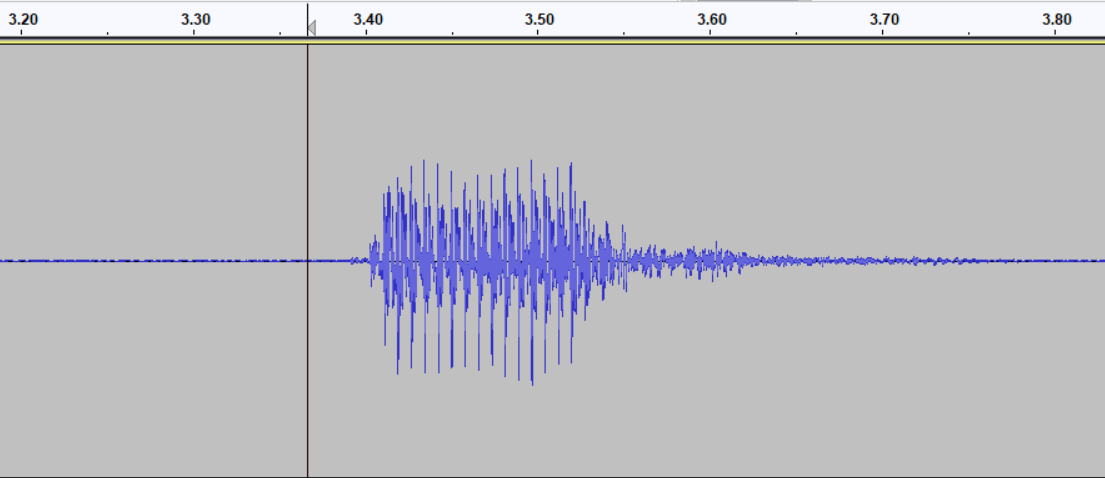
\includegraphics[width=9.5cm]{nsmr/img/a.png}
    \end{center}
    \caption{「あ」の全体の波形}
    \label{fig:asaisho}
  % \end{minipage}
\end{figure}
図\ref{fig:asaisho}を拡大すると図\ref{fig:aato}の波形が見えます。よく見ると1つの波が周期的に繰り返されているのがわかります。つまり、これが「あ」の音の正体であり、「あ」の固有な波形であると言えます。
\begin{figure}[H]
  % \begin{minipage}{0.33\hsize}
    \begin{center}
      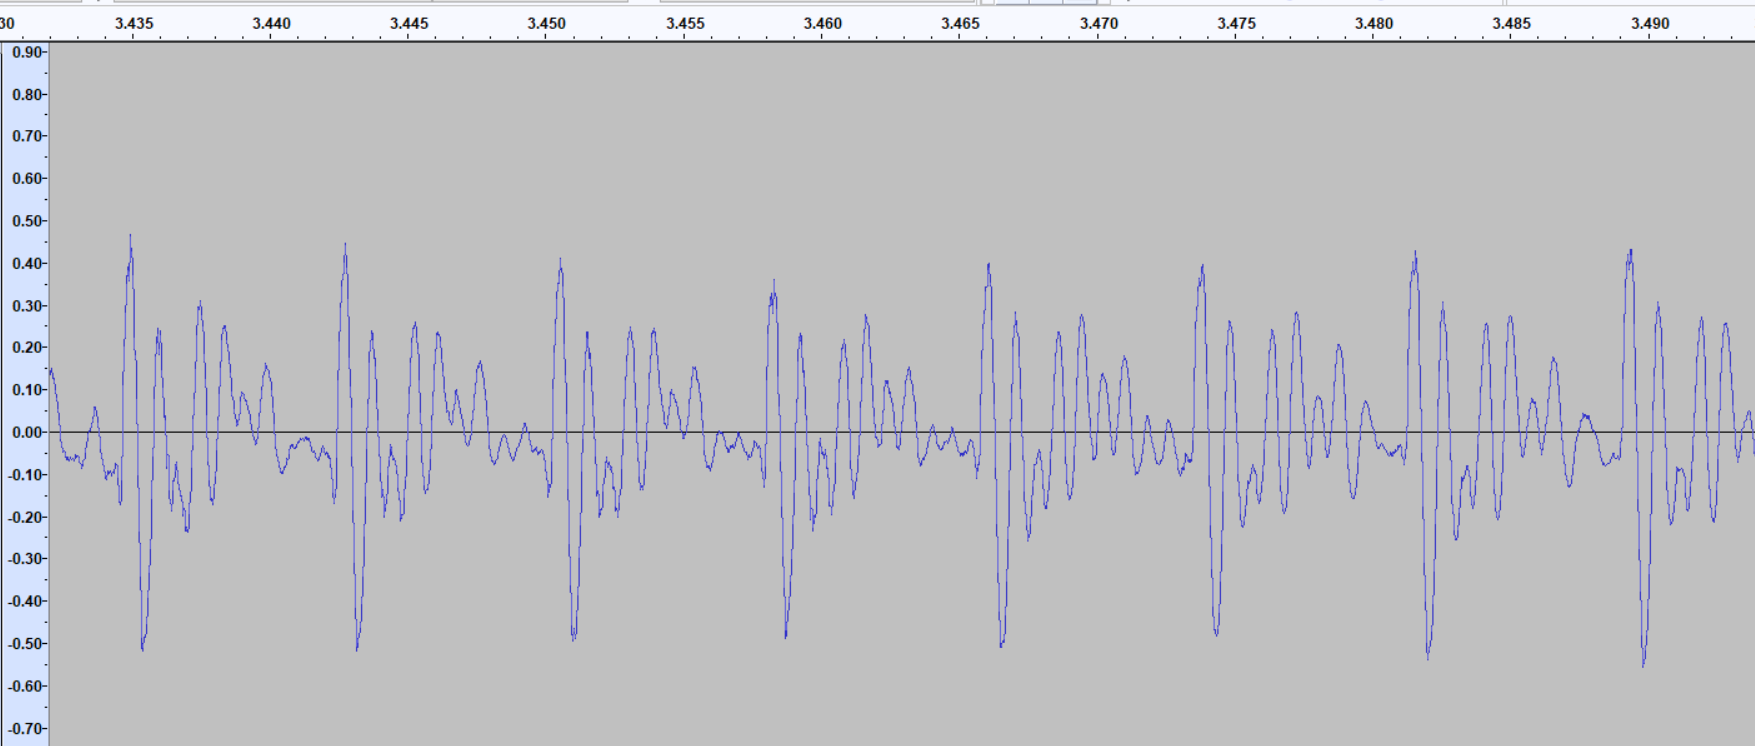
\includegraphics[width=9.5cm]{nsmr/img/a2.png}
    \end{center}
    \caption{「あ」の波形を拡大}
    \label{fig:aato}
  % \end{minipage}
\end{figure}

% - - - - - - - - - - - - - - - - - - -
\if0
\section{人間の耳}
%
\subsection{耳の構造}
人間の耳は複雑な形をしていて、聴覚は空気の音圧変化を耳で感じ取っています。\par
耳は外耳、中耳、内耳から成っています。もっと細かく機能別に分けると外耳は耳介と外耳道、内耳は三つの耳小骨(ツチ骨とキヌタ骨とアブミ骨)と鼓膜に分けられ、内耳は蝸牛と呼ばれる複雑な器官を持っています。
\begin{figure}[H]
  \centering
  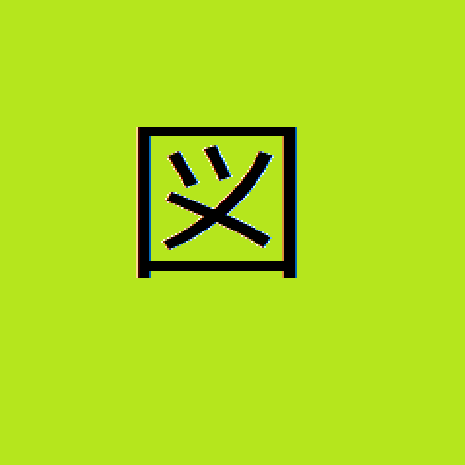
\includegraphics[width=5cm]{nsmr/img/zu.png}
  \caption{耳1}
\end{figure}

%
\subsection{耳の各部位の機能}
\begin{itemize} %
  \item 外耳・・・耳介と外耳道\\
  人間の耳は複雑な形をしています。なぜこのような耳介はそのような形をしているのでしょうか?\\
  正解の1つは音を集めるためです.。耳介は外耳道に音を集める役割をしています。前方からの音が聞こえにくい時に後方から耳に手を手の平が前になるように被せる動作をすると聞こえやすくなりますよね。\\
  二つ目の答えは耳介の凹凸構造により音源の方向を認知させる役割です。\\
  外耳には外耳道も含まれており、外耳道は直径0.7cm、奥行2.7cmで奥は鼓膜で閉じられています。外耳道の特徴は外耳道は約3kHzで共振し、音圧を10dB程度上昇させます。
  \item 中耳\\
  中耳の鼓膜は厚さ0.1mm、投影面積が約$55mm^2$の薄いロート状の膜です。\\
  耳小骨の役割は鼓膜の振動を内耳に中継することです。
  \item 内耳\\
  内耳は2回転+$3/4$回転している蝸牛の内部にあります。\\
  蝸牛\\
  蝸牛は内部がリンパ液で満たされていて、全長は約3cmです。\\
  蝸牛では鼓膜の振動を電気信号に変換します。蝸牛の内部はやや複雑な構造になっていて、基底膜によって前庭階と鼓室階に仕切られています。そして、それらは蝸牛の先端にある蝸牛孔でつながっています。\\
  鼓膜の振動は前庭窓を通して蝸牛に伝わり、内部を満たしたリンパ液を振動させます。こうしたリンパの振動は、前庭階から蝸牛孔を経由して鼓室階に伝わり、最終的に蝸牛窓に到達します。前庭窓と蝸牛窓は膜状のふたになっています。耳小骨の振動によって前庭窓が内部に押されると蝸牛窓は外部に押され、前庭窓が外部に引っ張られると蝸牛窓は内部に引っ張られるように動きます。
  \begin{figure}[H]
    \centering
    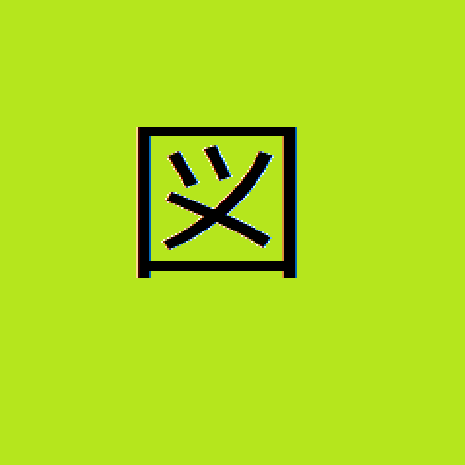
\includegraphics[width=5cm]{nsmr/img/zu.png}
    \caption{蝸牛}
  \end{figure}
  %
  \begin{figure}[H]
    \centering
    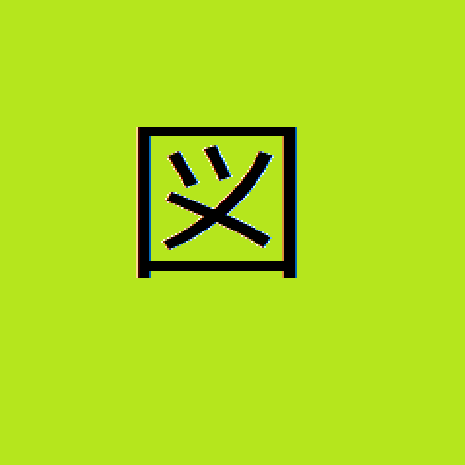
\includegraphics[width=5cm]{nsmr/img/zu.png}
    \caption{蝸牛断面}
  \end{figure}

\end{itemize} %
聴覚器官には、鼓膜の振動を効率よく蝸牛窓に伝える仕組みが備わっています。\\
1つは鼓膜と前庭窓の面積比は17:1になっていて、これにより鼓膜の振動が17倍に増幅されます。もう1つは耳小骨はツチ骨とキヌタ骨の長さの比が1.3:1になっていて、ツチ骨とキヌタ骨の連結部位を支点なり、てことして働くため鼓膜の振動が1.3倍に増幅します。\\
以上の二つが組み合わさることで鼓膜に届いた音は17\times1.3=22倍に増幅されて蝸牛窓に伝わります。
\fi
% - - - - - - - - - - - - - - - - - - -


%%
\section{イヤホンの世界(おまけ)}
おまけとしてここからはイヤホンの世界をお届けします(笑)。

%
\subsection{イヤホンの形の分類}
イヤホンの形状の種類は大きく2つに分けられます。
\begin{itemize}
  \item カナル型
  \item インナーイヤー型
\end{itemize}
カナル型イヤホンは耳栓を耳に装着するのと同じように耳に装着するタイプのイヤホンです。特徴としては、イヤホンのドライバー部分と鼓膜が近いので、音を綺麗に聞き取れることと、
イヤーチップがあるので耳に密着させることができ、外部の音を遮音することができるタイプのイヤホンです。
欠点はイヤーチップが耳に密着するので長時間イヤホンをつけていると、耳が痛くなってしまいます。\par
インナーイヤー型イヤホンとは耳の耳介にイヤホンを装着するタイプのイヤホンです。特徴はイヤホンと外耳道の入口との間に空間ができるので、外の音が聞こえやすいことです。欠点としては、外音を取り込んでしまうのを防ぐのに音量を上げすぎてしまいうことです。
音量が大きい状態に慣れてしまうと難聴になりやすくなってしまいます。
\begin{figure}[H]
  %
  \begin{minipage}{0.48\hsize}
    \begin{center}
      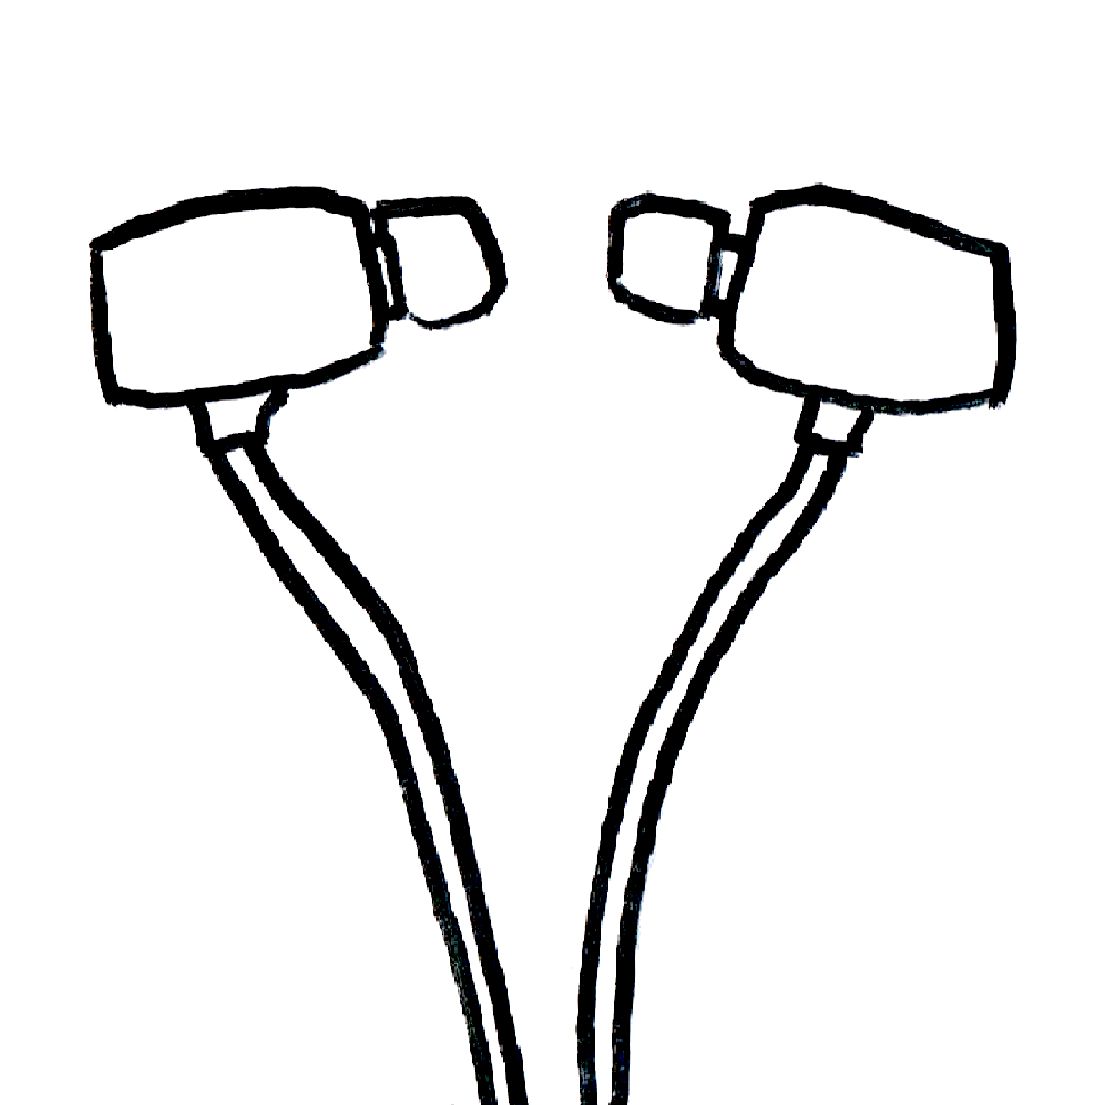
\includegraphics[height=3cm]{nsmr/img/kanaru.png}
    \end{center}
    \caption{カナル型イヤホン}
    \label{fig:kanaru}
  \end{minipage}
  %
  \begin{minipage}{0.48\hsize}
    \begin{center}
      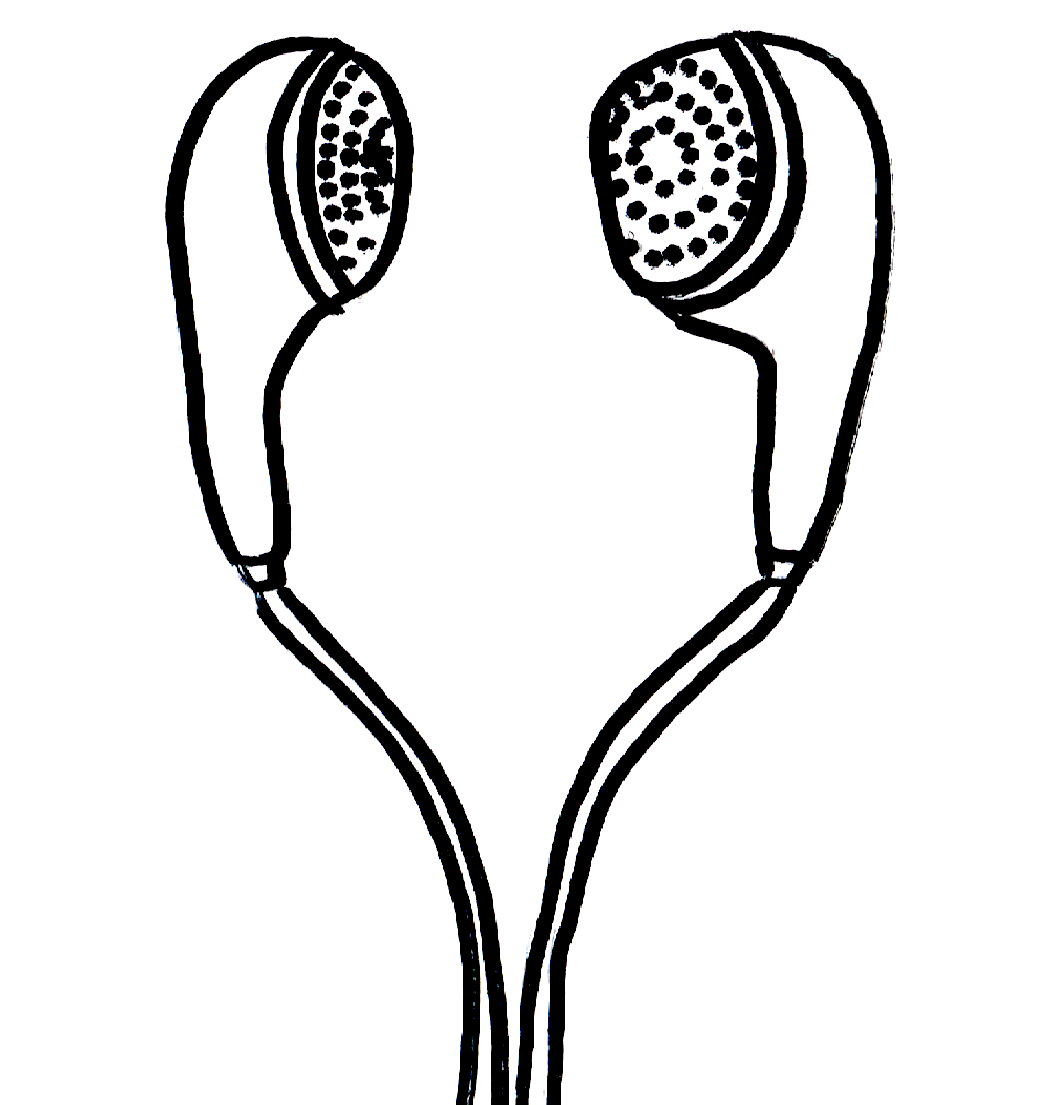
\includegraphics[height=3cm]{nsmr/img/inear.png}
    \end{center}
    \caption{インナーイヤー型イヤホン}
    \label{fig:innia}
  \end{minipage}
  %
\end{figure}

%
\newpage
\subsection{イヤホンのドライバー}
イヤホン内の音を出す部分をドライバーといいます。
ドライバーにはダイナミック型とバランスドアーマチュア型の2種類あります。\par
\begin{itemize}
  \item ダイナミック型
  \item バランスドアーマチュア型(BA型)
\end{itemize}
最近ではそれらのドライバーを組み合わせたハイブリッド型のイヤホンもありますが、すべてのイヤホンにはダイナミック型かバランスドアーマチュア型のどちらかが必ず使われています。
ではそれぞれのドライバーの特徴を見ていきましょう。\par
ダイナミック型イヤホンは1つのドライバーで再生できる音の周波数帯域が広く、低音を鳴らすのが
得意なイヤホンです。現在はイヤホンのドライバーの主流となっていて、
比較的安価で手に入るイヤホンにはダイナミック型のドライバーが搭載されています。
もちろん、高い再生能力や表現力があるダイナミック型のドライバーもたくさんあるので、ダイナミック型のイヤホン
だから音が良くないということは全くありません。\par
バランスドアーマチュア型イヤホンは1つのドライバーで再生できる音の周波数帯域が狭く、中音と高音を鳴らす
のが得意なイヤホンです。小型のドライバーであり、ドライバー内部の構造がダイナミック型に比べて複雑
なので、バランスドアーマチュア型のドライバーは簡単に作ることができません。
よって、バランスドアーマチュア型のドライバーは価格が高い傾向があります。それに加えて1つ1つのドライバーの周波数帯域が狭い
ことを補うために、複数のバランスドアーマチュア型のドライバーを搭載することも多いのでさらに価格は高くなります。
以上のことより、バランスドアーマチュア型のドライバーを搭載したイヤホンはダイナミック型のイヤホンに比べてマイナーな存在になっています。
しかし、ボーカルの声は中音に属するので声を重視にする人にはぜひ1度、バランスドアーマチュア型のドライバーを
搭載したイヤホンの音を聴いていただきたいです。


% 参考文献
\sanko
\begin{enumerate}
  \item 青木直史 (2014), 『ゼロからはじめる音響工学』,講談社.
  \item 久保和宏ほか(2009), 『音響学ABC』, 技報堂出版.
  \item 鈴木陽一ほか・日本音響学会編(2011), 『音響工学入門』, コロナ社.
\end{enumerate}


\end{document}
%
% ファイトだよ!
%